\documentclass{article}
\usepackage[utf8]{inputenc}
\usepackage{graphicx}
\usepackage{amsmath, amsthm, amsfonts, amssymb, amscd}
\usepackage{setspace, fancyhdr, float, xfrac, longtable, cite}
\usepackage{wrapfig, lscape, rotating, epstopdf, url}
\usepackage{array, booktabs, listings, latexsym}
\usepackage{tikz, standalone, calc}
\usetikzlibrary{shapes,arrows, decorations.markings}
%====================New Thm Declarations====================
\newtheorem{Thm}{Theorem}
\newtheorem{Cor}{Corollary}
\newtheorem{Lem}{Lemma}
\newtheorem{Prop}{Proposition}
\newtheorem{Def}{Definition}
\newtheorem{Exa}{Example}
\newtheorem{Asmpt}{Assumption}
\newcommand{\R}{\mathbb{R}}
\newcommand{\comment}[1]{}
\newtheorem{theorem}{Theorem}
\newtheorem{lemma}{Lemma}[section]
\newtheorem{remark}{Remark}[section]
\newtheorem{corollary}{Corollary}[section]
\newtheorem{proposition}{Proposition}[section]
\newtheorem{conjecture}{Conjecture}[section]
\newtheorem{example}{Example}[section]
\newtheorem{definition}{Definition}[section]
\newcommand{\eop}{\hfill $\sqcap\!\!\!\!\sqcup$} % end of proof
\newtheorem{Rem}{Remark}

%====================BEGIN DOCUMENT====================
\begin{document}
\title{Kernel Differential Observer}
\author{Basharnavaz Khan}
\maketitle

\begin{abstract}
This document contains the notes for the Master's thesis of Basharnavaz Khan. It is written here instead of the ETS format since this renders better readability.
\end{abstract}

\tableofcontents
\section{Introduction Motivation, Literature Review}
\subsection{Introduction}
Engineers are often interested in controlling the behaviour of their surroundings or a part of it, often referred to as a 'system' in order to provide desirable results in domains such as transportation manufacturing etc. In order to do so, engineers develop control systems which are interconnected components forming a system configuration that will provide a desired system response \cite{dorf_control_book}. These components are usually actuators, micro-controllers and power electronics that drive the actuators and software which contains the logic or algorithms which determine the actuation signals. \\As time progressed, the systems have become more complicated with multiple interrelated variables are needed to exhibit the behaviour. To control these systems there may be more than one actuator which attempts to make the system or plant have the desired behaviour and the control systems used to control such systems are called Multiple-variable control system. Most advanced control systems use the output of the plant of the system to be controlled as an important criteria to compute the subsequent control signals to the system. These type of control systems are called Closed Loop Control systems. Usually there is an error in the measurement of the plant output, known as measurement noise, which is attempted to minimize by using filtering algorithms that aid the control systems by providing more accurate information compute the intended control signal. In some cases control systems employ the use of observers which estimate the state of the system or external disturbances that affect it. This thesis aims at developing an observer based on an algebraic estimator to observe external aerodynamic disturbances and compare it with a couple of other observers in the literature. 



\subsection{Literature Review}
Realtime implementation of kernel methods was not done before. Explore properties and develop theorems of kernel estimator to make realtime computation possible.Notice that the simulations run about NDO and STO had simple sinusoidal disturbances and the observers having the knowledge of the initial conditions. 

\subsubsection{Nonlinear Disturbance Observer}
Nonlinear Disturbance Observer (NDO) is an asymptotic observer which was described and analysed in [cite NMHJ2018] and applied to the quadrotor system in [nuradeen]. The translational disturbances which affect the position of the quarotor is is described by the following equations: 
\begin{equation}
\begin{split}
\label{eq5:a}
\dot{z}_p &= -L_pz_p - L_p[L_p\dot{p}+G+\frac{1}{m}U_p ]\\
\hat{d}_p&=z_p + L_p\dot{p}
\end{split}
\end{equation}
where $U_p=R(\Theta) e_3 U_1$, $\widehat{d}_p$ is the estimate of translational disturbance,  $z_p$ is the state vector of the observer and $L_p=l_p I_{3 \times 3}, l_p >0$ are the gains of the observer which need to be tuned. 
The rotational disturbances which affect the orientation of the quadrotor is described by equations which have a similar form, 
\begin{equation}
\begin{split}
\label{eq5:b}
\dot{z}_\Theta &= -L_\Theta z_\Theta - L_\Theta[L_\Theta\dot{\Theta}+\Phi(\Theta,\dot{\Theta}) - U_\Theta] \\
\hat{d}_\Theta&=z_\Theta + L_\Theta\dot{\Theta}
\end{split}
\end{equation}
where $U_\Theta=\Psi(\Theta)[U_2\ \ U_3\ \ U_4]^T$, and $\widehat{d}_\Theta$ is the estimation of the rotational disturbance. The variable $z_\Theta$ is the state vector of the observer, and $L_\Theta=l_\Theta I_{3 \times 3}, l_\Theta >0$, are the observer gain matrices to be tuned.

For the purposes of brevity, only the theorems or propositions are mentioned here without their proofs. 

\subsubsection{Supertwisting Observer}


\subsection{Objectives}
Autonomous control systems rely on observers to estimate external disturbances in the system being controlled. Signal differentiation plays a crucial role in construction of non-linear disturbance observers. In this thesis, the student aims to compare three different disturbance estimation approaches for the purpose of constructing non-linear controllers for dynamical systems. Specifically, the nonlinear disturbance observers will be employed to estimate aerodynamic forces during quadrotor flights. \\
\textbf{Justification:} The thesis will focus on the development of kernel based algebraic differentiators of signals for estimation of disturbances from observation of the system inputs and outputs. A comparison of existing methods for
disturbance estimation will be carried out by way of simulations.  
The project will focus on development and implementation of algebraic observers on microcontrollers with limited processing abilities. It is envisioned that the example system will be a quadcopter.\\
\textbf{Methodologie}: The kernel based algebraic differentiators will employ a fourth order LTI structure over a moving window in conjunction with dynamic ridge regression. 
The performance of three different observers will be compared in close loop with a tracking control of a quadrotor. The other observers in the study are:
i) the nonlinear disturbance observer presented in [NuradeenSlidingMode2018] [NuradeenBackstepping2018]
ii) a super-twisting sliding mode observer
As mentioned above, based on the literature survey and preliminary simulations, the bottleneck in implementing algebraic estimators in practical systems is the computational effort, which several microcontrollers are not able provide.
The following steps will be made towards achieving the objectives of this project: 
\begin{itemize}
\item Development: Signal differentiators would be developed based on algebraic differentiation. 
\item Simulation: Comparison of methods found in literature and the one developed in simulations. The simulations will help in estimating the performance of the different observers mentioned. It is intended that the simulations will be carried out in MATLAB and Python
\item Practical Implementation: For the current project, a Parrot Mini-drone Rolling Spider quadcopter is chosen. This quadcopter has a MATLAB/Simulink interface which makes it easy to carryover simulation codes to the drone implementation. The drone has data logging capabilities which will make estimation performance analysis convenient. The student realizes that this will potentially involve several other tasks like inspecting C or C++ code which needs to be deployed in the hardware implementation.
\end{itemize}
	 
Tools: 
\begin{itemize}
\item MATLAB/Simulink: Primarily intended for simulations, Simulink interface with Parrot Mini-drone enables for a smoother workflow.
\item Python: Due to the ability to quickly prototype algorithms, Python provides a good option to test out different optimization
\item Parrot Mini-drone Rolling Spider: This would be practical framework on which estimation algorithms would be evaluated. 
\item C/C++: Software implementations on the drone would be in the C or C++ languages. 
Editors for the above languages are: PyCharm 2.0, Eclipse, Atom
\end{itemize}

\subsection{Thesis Organization}


\section{Quadcopter Model}
The quadcopter is an Unmanned Aerial Vehicle (UAV) under the class of Micro Air Vehicles(MAV). Historically research has been carried out on these class of aerial vehicles due to the advantages of flying in narrow or difficult to access areas while offering vertical take-off and landing capabilities. 
\begin{figure}
\centerline{\documentclass{standalone}

\usepackage{tikz}
\usetikzlibrary{shapes,arrows, decorations.markings}

\begin{document}
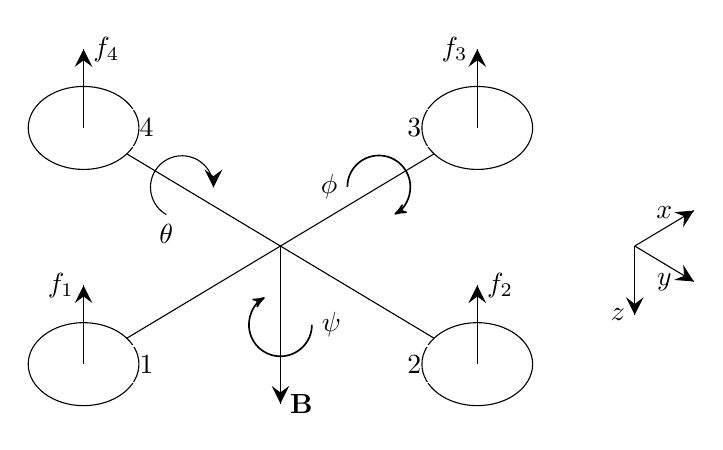
\begin{tikzpicture}
	\tikzstyle{prop} = [draw, ellipse, align=center, minimum width=4em, minimum height=3em]
	\tikzstyle{big_arrow} = [decoration={markings,mark=at position 1 with {\arrow[scale=2,>=stealth]{>}}},postaction={decorate}]
	% Prop nodes
	\node[prop, align=right] (1) at (0,0) {};
	\node[prop, align=left] (2) at (5,0) {};
	\node[prop, align=left] (3) at (5,3) {};
	\node[prop, align=right] (4) at (0,3) {};
	% Label props
	\node[draw=white, rectangle] at (0.8,0) {1};
	\node[draw=white, rectangle] at (4.2,0) {2};
	\node[draw=white, rectangle] at (4.2,3) {3};
	\node[draw=white, rectangle] at (0.8,3) {4};
	
	% Draw 
	% Connect props
	\draw [-] (1) -- node [midway, above] {} (3);
	\draw [-] (2) -- node [midway, above] {} (4);
		
	%Body Weight arrow 
	\draw [big_arrow] (2.5,1.5) -- node [at end, right] {\textbf{B}} (2.5,-0.5);
	% Prop thrust arrows
	\draw [big_arrow] (0,0) -- node [at end, left] {$f_1$} (0,1);
	\draw [big_arrow] (5,0) -- node [at end, right] {$f_2$} (5,1);
	\draw [big_arrow] (5,3) -- node [at end, left] {$f_3$} (5,4);
	\draw [big_arrow] (0,3) -- node [at end, right] {$f_4$} (0,4);
	
	% Draw arcs	
	\draw[big_arrow] (1.05,1.9) arc[radius=0.4, start angle=240, end angle=0] node[at start, below]{$\theta$};
	\draw[->,>=stealth',semithick] (3.35,2.25) arc[radius=0.4, start angle=180, end angle=-60] node[at start, left]{$\phi$};
	\draw[->,>=stealth',semithick] (2.9,0.5) arc[radius=0.4, start angle=0, end angle=-240] node[at start, right]{$\psi$};
	
	% Draw axes
	\draw [big_arrow] (7,1.5) -- node [midway, above] {$x$} (7.75,1.95);
	\draw [big_arrow] (7,1.5) -- node [midway, below] {$y$} (7.75,1.05);
	\draw [big_arrow] (7,1.5) -- node [at end, left] {$z$} (7,0.625);
	
\end{tikzpicture}

\end{document}}
\caption{Quadcopter model}
\label{quad_red_balls}
\end{figure}

\subsection{Flight Principle}
The flight principles of a quadcopter has been described in \cite{RN71} and many other works.
A quadcopter has four rotors positioned on its arms of equal lengths. The motors are numbered as No. 1 to No. 4, with opposite motors rotating in the same direction, i.e. No. 1 and No.3 rotate counter-clockwise direction and No. 2 and No.4 rotate in clockwise direction. The rotation of the motors provides the upward thrust against the gravity to keep the quadcopter in air. Rotation around an axis is obtained by rotational speed difference between the motors that are placed perpendicular to it. For instance, rotation around the X-axis is caused by the moment around the X-axis generated by the difference of rotational speed between motors No. 2 and No. 4. which are placed perpendicular to the X-axis. Rotation around the Y-axis is caused by a similar action. The rotation of the rotors exerts a torque on the quadcopter frame, due setting the airflow in rotation. The opposing direction of rotation of the motors maintain yaw stability, and a difference in rotation of motor causes yaw or rotation around the Z-axis.\\\ Insert figure of quadcopter.
\subsection{Dynamic Model}
The dynamic model has been described in previous works like \cite{hoffmann2007quadrotor}, \cite{zheng2014second} and \cite{alexis2012model}. The notation is similar as the one in the works to maintain consistency. 
The dynamics are considered in two frames, the body frame $(\mathcal{B})$ and the earth frame $(\mathcal{I})$. The position of the quadcopter in the inertial frame $(\mathcal{I})$ is the position of the center of the quadrotor's center of mass denoted by the vector $p=[x,y,z]^{T}$. The linear velocities and accelerations in the earth-frame are given by $\dot{p}=[\dot{x},\dot{y},\dot{z}]$, and $\ddot{p}=[\ddot{x},\ddot{y},\ddot{z}]$. 


Similarly, the attitude of the quadrotor in the inertial frame $(\mathcal{I})$, also known as the attitude of the quadrotor $(\Theta)$ is denoted by the vector, $\Theta=[\psi,\theta,\phi]$. The three components of this vector are Euler angles yaw ($-\pi<\psi<\pi$), pitch ($-\frac{\pi}{2}<\theta<\frac{\pi}{2}$), and roll ($-\frac{\pi}{2}<\phi<\frac{\pi}{2}$). The angular velocity of roll, pitch and yaw is defined as $\Omega=[\Omega_p,\Omega_q,\Omega_r]^T$ with respect to the body-fixed frame $(\mathcal{B})$, and $\ddot{\Theta}=[\ddot{\phi},\ddot{\theta},\ddot{\psi}]$ with respect to the inertia reference frame $\mathcal{I}$. The relation between $\dot{\Theta}$ and $\Omega$ is, 
\begin{equation}
\Omega=M(\Theta)\dot{\Theta}
\end{equation}
Where $M$ is given by, 
\begin{equation*}
M(\Theta)=
\left[\begin{array}{ccc}
1 & 0 & -S_{\theta} \\
0 & C_{\phi} & S_{\phi}C_{\theta}  \\
0 & -S_{\phi} & C_{\phi}S_{\theta}
\end{array}\right]
\end{equation*}
The functions $S_{(.)}$ and $C_{(.)}$ denote the $sin(.)$ and $cos(.)$ functions respectively. The rotation matrix which gives the kinematic relation for transformation between the body-fixed reference frame $\mathcal{B}$ and the inertial reference $\mathcal{I}$ This is denoted by $R$,
\begin{equation}
R(\Theta)=
\left[\begin{array}{ccc}
C_{\theta}C_{\psi} & S_{\phi}S_{\theta}C_{\psi}-C_{\phi}S_{\psi} & C_{\phi}S_{\theta}C_{\psi}+S_{\phi}S_{\psi} \\
C_{\theta}S_{\psi} & S_{\phi}S_{\theta}S_{\psi}+C_{\phi}C_{\psi} & C_{\phi}S_{\theta}S_{\psi}-S_{\phi}c_{\psi}  \\
-S_{\theta}  & S_{\phi}C_{\theta}  & C_{\phi}C_{\theta}
\end{array}\right]
\end{equation} 
For the purpose of estimation and control the quadrotor system is viewed as a subsystems, translational, the linear motion of the center of mass of the quadcopter, and, rotational, the attitude of the quadcopter. The equations of motion in the inertial frame $\mathcal{I}$ are expressed as,
\begin{subequations} \label{eq:dynamic_basic}
\begin{align} 
\ddot{p} &=\frac{1}{m}R(\Theta)F_{prop}-G+d_{p}(t) \label{eq:dynamic_basic_translation} \\
\ddot{\Theta} &=(IM(\Theta))^{-1}[T_{prop}-IN(\Theta,\dot{\Theta}) \nonumber \\
& \ \ -\Omega\times I\Omega-T_g]+d_{\Theta}(t)\nonumber\\
&=\Phi(\Theta,\dot{\Theta})+\Psi(\Theta) T_{prop}+d_{\Theta}(t)
 \label{eq:dynamic_basic_rotation}
\end{align}
\end{subequations}
where $N(\Theta,\dot{\Theta})$ is given by
\begin{equation*}
N(\Theta,\dot{\Theta})=
\left[\begin{array}{c}
-C_{\theta}\dot{\theta}\dot{\psi} \\
-S_{\phi}\dot{\phi}\dot{\theta}+C_{\phi}\dot{\phi}\dot{\psi} -S_{\phi}S_{\theta}\dot{\theta}\dot{\psi}\\
-C_{\phi}\dot{\phi}\dot{\theta}-S_{\phi}C_{\theta}\dot{\phi}\dot{\psi}-C_{\phi}S_{\theta}
\end{array}\right]
\end{equation*}
The resultant torque due to gyroscopic effects is given by, 
\begin{align}
T_d=\sum_{i=1}^{4}\Omega\times J_r[0,0,(-1)^{i+1}\omega_i]^T
\end{align}
where $J_r$ is the moment of inertia of each rotor and $\omega_i, i=1,2,3,4$ is the rotary speed of each motor.\\
$\Psi(\Theta)$ and $\Phi(\Theta,\dot{\Theta})$ are defined as
\begin{align*}
\Psi(\Theta)&=(IM(\Theta))^{-1}\\
\Phi(\Theta,\dot{\Theta})&=
-(IM(\Theta))^{-1}[IN(\Theta,\dot{\Theta}) -\Omega\times I\Omega-T_g]
\end{align*}

\textbf{REWRITE} The rotation of the propellers generates a thrust and a corresponding drag force. Assuming the force is proportional to the square of the motor speed \textbf{REWRITE}\\


The equations \eqref{eq:dynamic_basic_translation} and \eqref{eq:dynamic_basic_rotation} can be written as,

\begin{align}\label{eq:quad_dyanmics}
\begin{aligned}
\ddot{\phi}&=r_1\dot{\theta}\dot{\psi}-r_2\dot{\theta}w+q_1U_2+d_\phi\\
\ddot{\theta}&=r_3\dot{\phi}\dot{\psi}+r_4\dot{\phi}w+
q_2U_3+d_\theta\\
\ddot{\psi}&=r_5\dot{\theta}\dot{\phi}+q_3U_4+d_\psi\\
\ddot{x}&=(C_{\phi}S_{\theta}C_{\psi}+S_{\phi}S_{\psi})\frac{1}{m}U_1+d_x\\
\ddot{y}&=(C_{\phi}S_{\theta}S_{\psi}-S_{\phi}C_{\psi})\frac{1}{m}U_1+d_y\\
\ddot{z}&=-g+(C_{\phi}C_{\theta})\frac{1}{m}U_1+d_z
\end{aligned}
\end{align}
%form as $\dot{X}=f(X,U)$ 
where $[U_{1},U_{2},U_{3},U_{4}]^{T}$= $[T, T_{prop}]^T$ is the input vector.
\begin{align*}
\begin{aligned}
r_{1}&=\frac{I_{y}-I_{z}}{I_{x}},
r_{2}=-\frac{J_{r}}{I_{x}},
r_{3}=\frac{I_{z}-I_{x}}{I_{y}},
r_{4}=\frac{J_{r}}{I_{y}},\\
r_{5}&=\frac{I_{x}-I_{y}}{I_{z}},
q_{1}=\frac{h}{I_{x}},
q_{2}=\frac{h}{I_{y}},
q_{3}=\frac{1}{I_{z}}
\end{aligned}
\end{align*}\\

\subsection{Parameter Identification}
This is the identification of the parameters of the quadcopter. 
This is different than the parameter identification that will be shown in KDO, where the kernel parameters identified are used for the estimation of the state and the higher derivatives. 

\section{Kernel Differential Observer}
During a flight a quadrotor goes through uncertainties not only due to modeling errors but also due to aerodynamic disturbances. To achieve the best flight performances, and improve the overall robustness and stability of the control system, observers are employed to estimate the matched and unmatched disturbances in attempt that the control system if aware of the magnitude and nature of these disturbances would be able to eliminate the effect of these disturbances on the quadrotor system. In this thesis, the author develops a novel observer based on the Kernel differentiation techniques and compares it with observers found in the literature. The observer developed is called, Kernel Differential Observer, and compared against Nonlinear Disturbance Observer and Supertwisting Observer. 


\subsection{Estimation Objective}
Assume that the position, $p$, and the attitude, $\Theta$, of the quadrotor with respect to the inertia reference frame $\mathcal{I}$ are accessible for measurement with measured trajectories $p^{M}$ and $\Theta^{M}$. 
With the measured system output and no information on the initial estimate of the system, methods from the literature (Praveen's paper) are employed to obtain the best accuracy estimates of the full state of the quadrotor system.

Considering (the dynamic equation numbers), the objective is to design an observer for each subsystem (positional and rotational) separately, in order to obtain the best possible estimate of the external disturbances to the quadrotor system so that the controller makes the state variables [$p,\psi$] attain and follow their desired reference counterparts [$p_d,\psi_d$].

\subsection{Local Surrogate Model}
Explain how the local surrogate model works. Higher order surrogate models are much better suited for motion prediction. 

%\subsection{Kernels Representation}
May have to include a note on regression. 
Is regression needed? If regression is not used then there would not be any need for optimization. Regression was initally used to smoothen out trajectories, it is observed by Walid that smoothening out trajectories decreases robustness of the associated controller. Therefore, not using regression might help in having better trajectory tracking. 


\subsection{Development of the Double-Sided Kernel for a 4th Order LTI System\cite{Shaunak_thesis}}
The Double sided Kernel approach was developed in Kumar's thesis and it further developed for fourth order kernel representation in \cite{Shaunak_thesis} and is produced here for completeness. 

First, the fourth order LTI system is described and the deduction of a differential invariant is provided. Although the derivation is presented for a simple model, the method proceeds likewise for higher order systems. Its general validity has been proved by mathematical induction.
\subsubsection{A Differential Invariant of a LTI System}\label{differential-invariant}
We consider the following fourth order LTI SISO system:
\begin{equation}\label{eqn.42a}
\begin{split}
	\dot{x}(t) &= \mathbf{A}x(t)+\mathbf{B}u(t)\\
	y(t) &= \mathbf{C}x(t)
\end{split}
\end{equation}
where $\mathbf{A}$, $\mathbf{C}$, $x(t)$, $\dot{x}(t)$ and $y(t)$ are given as follows 
\begin{equation*}\label{eqn.42b}
	\mathbf{A} = \begin{bmatrix}
	0 & 1 & 0 & 0\\[0.3em]
	0 & 0 & 1 & 0\\[0.3em]
	0 & 0 & 0 & 1\\[0.3em]
	-a_0 & -a_1 & -a_2 & -a_3\\[0.3em]
	\end{bmatrix}
\end{equation*}
\begin{equation*}
\begin{split}
	\mathbf{B} = \begin{bmatrix}
	0 & 0 & 0 & 1 \\[0.3em]
	\end{bmatrix}^\intercal
\end{split}
\end{equation*}
\begin{equation*}\label{eqn.42c}
	\mathbf{C} = \begin{bmatrix}
	1 & 0 & 0 & 0 \\[0.3em]
\end{bmatrix}
\end{equation*}
\begin{equation*}\label{eqn.42d}
	x(t) = \begin{bmatrix}
	x_{1}(t)\quad x_{2}(t)\quad x_{3}(t)\quad x_{4}(t) \\[0.3em]
	\end{bmatrix}^\intercal
\end{equation*}
\begin{equation*}\label{eqn.42e}
	\dot{x}(t) = \begin{bmatrix}
	\dot{x}_{1}(t)\quad\dot{x}_{2}(t)\quad\dot{x}_{3}(t)\quad\dot{x}_{4}(t)\end{bmatrix}^\intercal
\end{equation*}
\begin{equation*}\label{eqn.42f}
	y(t) = x_1(t)
\end{equation*}
From \eqref{eqn.42a}, we get the following state equations:
\begin{equation}\label{eqn.42g}
	\begin{split}
	&\dot{x}_{1}(t) = x_2(t) = y^{(1)}(t)\\
	&\dot{x}_{2}(t) = x_3(t) = y^{(2)}(t)\\
	&\dot{x}_{3}(t) = x_4(t) = y^{(3)}(t)\\
	&\dot{x}_{4}(t) = -a_0x_1(t)-a_1x_2(t)-a_2x_3(t)-a_3x_4(t)+u(t) = y^{(4)}(t)\\
	\end{split}
\end{equation}
Using the relations in equation \eqref{eqn.42g}, we arrive at the required differential invariant:
\begin{equation}\label{eqn.43}	
\begin{split}
	y^{(4)}(t) + a_{3}y^{(3)}(t) + a_{2} y^{(2)}(t) + a_{1}y^{(1)}(t) + a_{0}y(t) = u(t)
\end{split}
\end{equation}
\subsubsection{Derivation of the Behavioral Model}
The double-sided kernel is derived for the general fourth order characteristic polynomial obtained in subsection \ref{differential-invariant} on an arbitrary interval $[a, b]$.\\

Two equations are obtained from \eqref{eqn.43}  by pre-multiplication of both sides of the equation by the factors $(\gamma-a)^4$ and $(b-\gamma)^4$, respectively :
\begin{equation}\label{eqn.44}	
\begin{split}
	\underbrace{(\gamma-a)^{4}y^{(4)}(t)}_\text{$T_1$} + \underbrace{a_{3}(\gamma-a)^{4}y^{(3)}(t)}_\text{$T_2$} + \underbrace{a_{2}(\gamma-a)^{4}y^{(2)}(t)}_\text{$T_3$} + \underbrace{a_{1}(\gamma-a)^{4}y^{(1)}(t)}_\text{$T_4$}\\ +\underbrace{a_{0}(\gamma-a)^{4}y(t)}_\text{$T_5$} - \underbrace{(\gamma-a)^{4}u(t)}_\text{$T_6$} = 0
\end{split}
\end{equation}
\begin{equation}\label{eqn.45}	
\begin{split}
	\underbrace{(b-\gamma)^{4}y^{(4)}(t)}_\text{$J_1$} + \underbrace{a_{3}(b-\gamma)^{4}y^{(3)}(t)}_\text{$J_2$} + \underbrace{a_{2}(b-\gamma)^{4}y^{(2)}(t)}_\text{$J_3$} + \underbrace{a_{1}(b-\gamma)^{4}y^{(1)}(t)}_\text{$J_4$}\\ +\underbrace{a_{0}(b-\gamma)^{4}y(t)}_\text{$J_5$} - \underbrace{(b-\gamma)^{4}u(t)}_\text{$J_6$} = 0
\end{split}
\end{equation}
Now, we integrate \eqref{eqn.44} and \eqref{eqn.45} four times, term-wise, on the respective intervals $[a, a+\tau]$ and $[b-\sigma, b]$ while assuming that $\tau$ and $\sigma$ are related by $a+\tau=b-\sigma$. Integration by parts is used whenever it allows to lower the degree of the derivative terms under the integrals and the result is then simplified algebraically before proceeding to the next integration. The procedure is illustrated step by step below.\\
Integrating $T_1$ in \eqref{eqn.44} once we get,
\begin{equation}\label{eqn.46}
\begin{split}
	&\int\limits_{a}^{a+\tau}(\gamma-a)^4 y^{(4)}(\gamma)\, \mathrm{d}\gamma\\
	& = (\gamma-a)^4 y^{(3)}(\gamma)\mid_a^{a+\tau} - \int\limits_{a}^{a+\tau} 4(\gamma-a)^3 y^{(3)}(\gamma)\, \mathrm{d}\gamma \\
	& =  \tau^4 y^{(3)}(a+\tau) - \bigg[ 4(\gamma-a)^3 y^{(2)}(\gamma) \mid_a^{a+\tau} - \int\limits_a^{a+\tau} 12(\gamma-a)^{2} y^{(2)}(\gamma) \mathrm{d}\gamma \bigg]\\
	& = \tau^4 y^{(3)}(a+\tau) - 4\tau^3 y^{(2)}(a+\tau) + 12(\gamma-a)^{2}y^{(1)}(\gamma) \mid_a^{a+\tau} - \int\limits_a^{a+\tau} 24(\gamma-a) y^{(1)}(\gamma)\, \mathrm{d}\gamma\\
	& = \tau^4 y^{(3)}(a+\tau) - 4\tau^3 y^{(2)}(a+\tau) + 12\tau^2 y^{(1)}(a+\tau) \\&\qquad{}- 24\bigg[(\gamma-a)y(\gamma)\mid_a^{a+\tau}-\int\limits_a^{a+\tau} 6 y(\gamma)\, \mathrm{d}\gamma\bigg]\\
	& = \tau^4 y^{(3)}(a+\tau) - 4\tau^3 y^{(2)}(a+\tau) + 12\tau^2 y^{(1)}(a+\tau) - 24\tau y(a+\tau)\\&\qquad{}+\int\limits_a^{a+\tau} 24 y(\gamma)\, \mathrm{d}\gamma
\end{split}
\end{equation}
Next, the upper limit on the integral is replaced by a \lq dummy variable\rq, i.e., we set $\gamma'=a+\tau$. The terms in \eqref{eqn.46} can then be written as:\vspace{\baselineskip}\\
$\tau^4 y^{(3)}(a+\tau) = (\gamma'-a)^4 y^{(3)}(\gamma')$\\
$4\tau^3 y^{(2)}(a+\tau) = 4(\gamma'-a)^3 y^{(2)}(\gamma')$\\
$12\tau^2 y^{(1)}(a+\tau) = 12(\gamma'-a)^2 y^{(1)}(\gamma')$\\
$24\tau y(a+\tau) = 24(\gamma'-a) y(\gamma')$\\
Now, integrating $T_1$ for the second time,
\begin{equation}\label{eqn.47}
\begin{split}
&\int\limits_{a}^{a+\tau}\int\limits_{a}^{\gamma'} (\gamma-a)^4 y^{(4)}(\gamma)\, \mathrm{d}\gamma \mathrm{d}\gamma'\\ 
& = \int\limits_{a}^{a+\tau}(\gamma'-a)^4 y^{(3)}(\gamma')\, \mathrm{d}  \gamma'- \int\limits_{a}^{a+\tau}4(\gamma'-a)^3 y^{(2)}(\gamma')\, \mathrm{d}\gamma' + \int\limits_{a}^{a+\tau} 12(\gamma'-a)^{2} y^{(1)}(\gamma')\, \mathrm{d}\gamma'\\
&\qquad{} - \int\limits_{a}^{a+\tau} 24(\gamma'-a) y(\gamma')\, \mathrm{d}\gamma' + \int\limits_{a}^{a+\tau}\int\limits_{a}^{\gamma'} 24 y(\gamma)\, \mathrm{d}\gamma \mathrm{d}\gamma'\\
& = \tau^{4}y^{(2)}(a+\tau) - 8\tau^{3}y^{(1)}(a+\tau) + 36\tau^{2}y(a+\tau) - \int\limits_{a}^{a+\tau}96(\gamma'-a)y(\gamma')\mathrm{d}\gamma'\\
&\qquad{} + \int\limits_{a}^{a+\tau}\int\limits_{a}^{\gamma'}24y(\gamma)\mathrm{d}\gamma\mathrm{d}\gamma' 
\end{split}
\end{equation}
Replacing the upper limit on the integral by a \lq dummy variable\rq, $\gamma''=a+\tau$ and integrating $T_1$ for the third time, we get,\\
\begin{equation}\label{eqn.48}
\begin{split}
&\int\limits_{a}^{a+\tau}\int\limits_{a}^{\gamma''}\int\limits_{a}^{\gamma'} (\gamma-a)^4 y^{(4)}(\gamma)\, \mathrm{d}\gamma \mathrm{d}\gamma'\mathrm{d}\gamma''\\ 
& = \int\limits_{a}^{a+\tau}(\gamma''-a)^4 y^{(2)}(\gamma'')\, \mathrm{d}  \gamma''- \int\limits_{a}^{a+\tau}8(\gamma''-a)^3 y^{(1)}(\gamma'')\, \mathrm{d}\gamma'' + \int\limits_{a}^{a+\tau}36(\gamma''-a)^{2} y(\gamma'')\, \mathrm{d}\gamma''\\
&\qquad{} - \int\limits_{a}^{a+\tau}\int\limits_{a}^{\gamma''} 96(\gamma'-a) y(\gamma')\, \mathrm{d}\gamma'\mathrm{d}\gamma'' + \int\limits_{a}^{a+\tau}\int\limits_{a}^{\gamma''}\int\limits_{a}^{\gamma'} y(\gamma)\, \mathrm{d}\gamma \mathrm{d}\gamma' \mathrm{d}\gamma''\\
& = \tau^{4}y^{(1)}(a+\tau) - 12\tau^{3}y(a+\tau) + \int\limits_{a}^{a+\tau}72(\gamma''-a)^{2}y(\gamma'')\mathrm{d}\gamma''\\&\qquad{} - \int\limits_{a}^{a+\tau}\int\limits_{a}^{\gamma''}96(\gamma'-a)y(\gamma')\mathrm{d}\gamma'\mathrm{d}\gamma''+ \int\limits_{a}^{a+\tau}\int\limits_{a}^{\gamma''}\int\limits_{a}^{\gamma'} 24 y(\gamma)\mathrm{d}\gamma\mathrm{d}\gamma'\mathrm{d}\gamma''
\end{split}
\end{equation}

Finally, replacing the upper limit on the integral by a \lq dummy variable\rq, $\gamma'''=a+\tau$ and integrating $T_1$ for the fourth time, we get,\\
\begin{equation}\label{eqn.49}
\begin{split}
&\int\limits_{a}^{a+\tau}\int\limits_{a}^{\gamma'''}\int\limits_{a}^{\gamma''}\int\limits_{a}^{\gamma'} (\gamma-a)^4 y^{(4)}(\gamma)\, \mathrm{d}\gamma \mathrm{d}\gamma'\mathrm{d}\gamma''\mathrm{d}\gamma'''\\ 
& = \int\limits_{a}^{a+\tau}(\gamma'''-a)^{4}y^{(1)}(\gamma''')\mathrm{d}\gamma''' -\int\limits_{a}^{a+\tau} 12(\gamma'''-a)^{3}y(\gamma''')\mathrm{d}\gamma'''\\&\qquad{} + \int\limits_{a}^{a+\tau}\int\limits_{a}^{\gamma'''}72(\gamma''-a)^{2}y(\gamma'')\mathrm{d}\gamma''\mathrm{d}\gamma'''- \int\limits_{a}^{a+\tau}\int\limits_{a}^{\gamma'''}\int\limits_{a}^{\gamma''}96(\gamma'-a)y(\gamma')\mathrm{d}\gamma'\mathrm{d}\gamma''\mathrm{d}\gamma'''
\\&\qquad{}+ \int\limits_{a}^{a+\tau}\int\limits_{a}^{\gamma'''}\int\limits_{a}^{\gamma''}\int\limits_{a}^{\gamma'} 24 y(\gamma)\mathrm{d}\gamma\mathrm{d}\gamma'\mathrm{d}\gamma''\mathrm{d}\gamma'''\\
&= \tau^{4}y(a+\tau)-\int\limits_{a}^{a+\tau}16(\gamma'''-a)^{3}y(\gamma''')\mathrm{d}\gamma'''+\int\limits_{a}^{a+\tau}\int\limits_{a}^{\gamma'''}72(\gamma''-a)^{2}y(\gamma'')\mathrm{d}\gamma''\mathrm{d}\gamma'''\\
&\qquad{} - \int\limits_{a}^{a+\tau}\int\limits_{a}^{\gamma'''}\int\limits_{a}^{\gamma''}96(\gamma'-a)y(\gamma')\mathrm{d}\gamma'\mathrm{d}\gamma''\mathrm{d}\gamma''' +
\int\limits_{a}^{a+\tau}\int\limits_{a}^{\gamma'''}\int\limits_{a}^{\gamma''}\int\limits_{a}^{\gamma'}24y(\gamma)\mathrm{d}\gamma\mathrm{d}\gamma'\mathrm{d}\gamma''\mathrm{d}\gamma'''
\end{split}
\end{equation}
\\Integrating term $T_2$ in \eqref{eqn.44} once, we get,
\begin{equation}
\begin{split}
	&\int\limits_{a}^{a+\tau}a_3(\gamma -a)^{4}y^{(3)}(\gamma)\mathrm{d}\gamma\\
	& = a_3(\gamma-a)^{4}y^{(2)}(\gamma)\mid_{a}^{a+\tau} - \int\limits_{a}^{a+\tau}4a_3(\gamma -a)^{3}y^{(2)}(\gamma)\mathrm{d}\gamma\\
	& = a_3\tau^{4}y^{(2)}(a+\tau) - \bigg[4a_3(\gamma-a)^{3}y^{(1)}(\gamma)\mid_{a}^{a+\tau}- \int\limits_{a}^{a+\tau}12a_3(\gamma-a)^{2}y^{(1)}(\gamma)\mathrm{d}\gamma\bigg]\\
	& = a_3\tau^{4}y^{(2)}(a+\tau) -4a_3\tau^{3}y^{(1)}(a+\tau) + 12a_3\tau^{2}y(a+\tau)-\int\limits_{a}^{a+\tau}24a_3(\gamma-a)y(\gamma)\mathrm{d}\gamma
	\end{split}
\end{equation}
Introducing the \lq dummy variable\rq, $\gamma'=a+\tau$ as done before, and integrating $T_2$ for the second time:

\begin{equation}
\begin{split}
	&\int\limits_{a}^{a+\tau}\int\limits_{a}^{\gamma'}a_3(\gamma -a)^{4}y^{(3)}(\gamma)\mathrm{d}\gamma\mathrm{d}\gamma'\\
	& = \int\limits_{a}^{a+\tau}a_3(\gamma'-a)^{4}y^{(2)}(\gamma')\mathrm{d}\gamma' - \int\limits_{a}^{a+\tau}4a_3(\gamma' -a)^{3}y^{(1)}(\gamma')\mathrm{d}\gamma' \\&\qquad{}+\int\limits_{a}^{a+\tau}12a_3(\gamma'-a)^{2}y(\gamma')\mathrm{d}\gamma' -\int\limits_{a}^{a+\tau}\int\limits_{a}^{\gamma'}24a_3(\gamma-a)y(\gamma)\mathrm{d}\gamma\mathrm{d}\gamma'\\
	& = a_3\tau^{4}y^{(1)}(a+\tau) - 8a_3\tau^{3}y(a+\tau) + \int\limits_{a}^{a+\tau}36a_3(\gamma'-a)^{2}y(\gamma')\mathrm{d}\gamma'\\ &\qquad{} -\int\limits_{a}^{a+\tau}\int\limits_{a}^{\gamma'}24a_3(\gamma-a)y(\gamma)\mathrm{d}\gamma\mathrm{d}\gamma'
\end{split}
\end{equation}
Integrating $T_2$ for the third time:
\begin{equation}
\begin{split}
	&\int\limits_{a}^{a+\tau}\int\limits_{a}^{\gamma''}\int\limits_{a}^{\gamma'}a_3(\gamma -a)^{4}y^{(3)}(\gamma)\mathrm{d}\gamma\mathrm{d}\gamma'\mathrm{d}\gamma''\\
	& = \int\limits_{a}^{a+\tau}a_3(\gamma''-a)^{4}y^{(1)}(\gamma'')\mathrm{d}\gamma'' - \int\limits_{a}^{a+\tau}8a_3(\gamma'' -a)^{3}y(\gamma'')\mathrm{d}\gamma''\\&\qquad{} +\int\limits_{a}^{a+\tau}\int\limits_{a}^{\gamma''}36a_3(\gamma'-a)^{2}y(\gamma')\mathrm{d}\gamma'\mathrm{d}\gamma'' -\int\limits_{a}^{a+\tau}\int\limits_{a}^{\gamma''}\int\limits_{a}^{\gamma'}24a_3(\gamma-a)y(\gamma)\mathrm{d}\gamma\mathrm{d}\gamma'\mathrm{d}\gamma''\\
	& = a_3\tau^{4}y(a+\tau) - \int\limits_{a}^{a+\tau}12a_3(\gamma''-a)^{3}y(\gamma'')\mathrm{d}\gamma'' + \int\limits_{a}^{a+\tau}\int\limits_{a}^{\gamma''}36a_3(\gamma'-a)^{2}y(\gamma')\mathrm{d}\gamma'\mathrm{d}\gamma''\\ 
	&\qquad{}-\int\limits_{a}^{a+\tau}\int\limits_{a}^{\gamma''}\int\limits_{a}^{\gamma'}24a_3(\gamma-a)y(\gamma)\mathrm{d}\gamma\mathrm{d}\gamma'\mathrm{d}\gamma''
\end{split}
\end{equation}
Integrating $T_2$ for the fourth time:
\begin{equation}
\begin{split}
	&\int\limits_{a}^{a+\tau}\int\limits_{a}^{\gamma'''}\int\limits_{a}^{\gamma''}\int\limits_{a}^{\gamma'}a_3(\gamma -a)^{4}y^{(3)}(\gamma)\mathrm{d}\gamma\mathrm{d}\gamma'\mathrm{d}\gamma''\\
	& = \int\limits_{a}^{a+\tau}a_3(\gamma'''-a)^{4}y(\gamma''')\mathrm{d}\gamma''' - \int\limits_{a}^{a+\tau}\int\limits_{a}^{\gamma'''}12a_3(\gamma'' -a)^{3}y(\gamma'')\mathrm{d}\gamma''\mathrm{d}\gamma'''\\ 	&\qquad{}+\int\limits_{a}^{a+\tau}\int\limits_{a}^{\gamma'''}\int\limits_{a}^{\gamma''}36a_3(\gamma'-a)^{2}y(\gamma')\mathrm{d}\gamma'\mathrm{d}\gamma''\mathrm{d}\gamma''' \\&\qquad{}-\int\limits_{a}^{a+\tau}\int\limits_{a}^{\gamma'''}\int\limits_{a}^{\gamma''}\int\limits_{a}^{\gamma'}24a_3(\gamma-a)y(\gamma)\mathrm{d}\gamma\mathrm{d}\gamma'\mathrm{d}\gamma''\mathrm{d}\gamma'''
\end{split}
\end{equation}
\\Integrating term $T_3$ in \eqref{eqn.44} once, we get,
\begin{equation}
\begin{split}
	&\int\limits_{a}^{a+\tau}a_2(\gamma-a)^{4}y^{(2)}(\gamma)\mathrm{d}\gamma\\
	&=a_2(\gamma-a)^{4}y^{(1)}(\gamma)\mid_{a}^{a+\tau} - \int\limits_{a}^{a+\tau}4a_2(\gamma-a)^{3}y^{(1)}(\gamma)\mathrm{d}\gamma\\
	&=a_2\tau^4y^{(1)}(a+\tau) - \bigg[4a_2(\gamma-a)^3y(\gamma)\mid_{a}^{a+\tau} - \int\limits_{a}^{a+\tau}12a_2(\gamma-a)^2y(\gamma)\mathrm{d}\gamma\bigg]\\
	&=a_2\tau^4y^{(1)}(a+\tau) -4a_2\tau^3y(a+\tau)+\int\limits_{a}^{a+\tau}12a_2(\gamma-a)^2y(\gamma)\mathrm{d}\gamma
\end{split}
\end{equation}
Integrating $T_3$ for the second time:
\begin{equation}
\begin{split}
	&\int\limits_{a}^{a+\tau}\int\limits_{a}^{\gamma'}a_2(\gamma-a)^{4}y^{(2)}(\gamma)\mathrm{d}\gamma\mathrm{d}\gamma'\\
	&=\int\limits_{a}^{a+\tau}a_2(\gamma'-a)^4y^{(1)}(\gamma')\mathrm{d}\gamma' -\int\limits_{a}^{a+\tau}4a_2(\gamma'-a)^3y(\gamma')\mathrm{d}\gamma'
	\\&\qquad{}+\int\limits_{a}^{a+\tau}\int\limits_{a}^{\gamma'}12a_2(\gamma-a)^2y(\gamma)\mathrm{d}\gamma\mathrm{d}\gamma'\\
	&=a_2\tau^{4}y(a+\tau)-\int\limits_{a}^{a+\tau}8a_2(\gamma'-a)^{3}y(\gamma')\mathrm{d}\gamma' + \int\limits_{a}^{a+\tau}\int\limits_{a}^{\gamma'}12a_2(\gamma-a)^2y(\gamma)\mathrm{d}\gamma\mathrm{d}\gamma'
\end{split}
\end{equation}
Integrating $T_3$ for the third time:
\begin{equation}
\begin{split}
	&\int\limits_{a}^{a+\tau}\int\limits_{a}^{\gamma''}\int\limits_{a}^{\gamma'}a_2(\gamma-a)^{4}y^{(2)}(\gamma)\mathrm{d}\gamma\mathrm{d}\gamma'\mathrm{d}\gamma''\\
	&=\int\limits_{a}^{a+\tau}a_2(\gamma''-a)^4y(\gamma'')\mathrm{d}\gamma'' -\int\limits_{a}^{a+\tau}\int\limits_{a}^{\gamma''}8a_2(\gamma'-a)^3y(\gamma')\mathrm{d}\gamma'\mathrm{d}\gamma''\\
	&\qquad{} + \int\limits_{a}^{a+\tau}\int\limits_{a}^{\gamma''}\int\limits_{a}^{\gamma'}12a_2(\gamma-a)^2y(\gamma)\mathrm{d}\gamma\mathrm{d}\gamma'\mathrm{d}\gamma''
\end{split}
\end{equation}
Integrating $T_3$ for the fourth time:
\begin{equation}
\begin{split}
	&\int\limits_{a}^{a+\tau}\int\limits_{a}^{\gamma'''}\int\limits_{a}^{\gamma''}\int\limits_{a}^{\gamma'}a_2(\gamma-a)^{4}y^{(2)}(\gamma)\mathrm{d}\gamma\mathrm{d}\gamma'\mathrm{d}\gamma''\mathrm{d}\gamma'''\\
	&=\int\limits_{a}^{a+\tau}\int\limits_{a}^{\gamma'''}a_2(\gamma''-a)^4y(\gamma'')\mathrm{d}\gamma''\mathrm{d}\gamma''' -\int\limits_{a}^{a+\tau}\int\limits_{a}^{\gamma'''}\int\limits_{a}^{\gamma''}8a_2(\gamma'-a)^3y(\gamma')\mathrm{d}\gamma'\mathrm{d}\gamma''\mathrm{d}\gamma'''\\
	&\qquad{} + \int\limits_{a}^{a+\tau}\int\limits_{a}^{\gamma'''}\int\limits_{a}^{\gamma''}\int\limits_{a}^{\gamma'}12a_2(\gamma-a)^2y(\gamma)\mathrm{d}\gamma\mathrm{d}\gamma'\mathrm{d}\gamma''\mathrm{d}\gamma'''
\end{split}
\end{equation}
\\Integrating term $T_4$ in \eqref{eqn.44} once, we get,
\begin{equation}
\begin{split}
	&\int\limits_{a}^{a+\tau}a_1(\gamma-a)y^{(1)}(\gamma)\mathrm{d}\gamma\\
	&=a_1(\gamma-a)^4y(\gamma)\mid_{a}^{a+\tau}-\int\limits_{a}^{a+\tau}4a_1(\gamma-a)^{3}y(\gamma)\mathrm{d}\gamma\\
	&=a_1\tau^4y(a+\tau) - \int\limits_{a}^{a+\tau}4a_1(\gamma-a)^3y(\gamma)\mathrm{d}\gamma
\end{split}
\end{equation}
\\Integrating $T_4$ for the second time:
\begin{equation}
\begin{split}
	&\int\limits_{a}^{a+\tau}\int\limits_{a}^{\gamma'}a_1(\gamma-a)^{4}y^{(1)}(\gamma)\mathrm{d}\gamma\mathrm{d}\gamma'\\
	&=\int\limits_{a}^{a+\tau}a_1(\gamma'-a)^4y(\gamma')\mathrm{d}\gamma' - \int\limits_{a}^{a+\tau}\int\limits_{a}^{\gamma'}4a_1(\gamma-a)^3y(\gamma)\mathrm{d}\gamma\mathrm{d}\gamma'
\end{split}
\end{equation}
\\Integrating $T_4$ for the third time:
\begin{equation}
\begin{split}
	&\int\limits_{a}^{a+\tau}\int\limits_{a}^{\gamma''}\int\limits_{a}^{\gamma'}a_1(\gamma-a)^{4}y^{(1)}(\gamma)\mathrm{d}\gamma\mathrm{d}\gamma'\mathrm{d}\gamma''\\
	&=\int\limits_{a}^{a+\tau}\int\limits_{a}^{\gamma''}a_1(\gamma'-a)^4y(\gamma')\mathrm{d}\gamma'\mathrm{d}\gamma'' - \int\limits_{a}^{a+\tau}\int\limits_{a}^{\gamma''}\int\limits_{a}^{\gamma'}4a_1(\gamma-a)^3y(\gamma)\mathrm{d}\gamma\mathrm{d}\gamma'\mathrm{d}\gamma''
\end{split}
\end{equation}
\\Integrating $T_4$ for the fourth time:
\begin{equation}
\begin{split}
	&\int\limits_{a}^{a+\tau}\int\limits_{a}^{\gamma'''}\int\limits_{a}^{\gamma''}\int\limits_{a}^{\gamma'}a_1(\gamma-a)^{4}y^{(1)}(\gamma)\mathrm{d}\gamma\mathrm{d}\gamma'\mathrm{d}\gamma''\mathrm{d}\gamma'''\\
	&=\int\limits_{a}^{a+\tau}\int\limits_{a}^{\gamma'''}\int\limits_{a}^{\gamma''}a_1(\gamma'-a)^4y(\gamma')\mathrm{d}\gamma'\mathrm{d}\gamma''\mathrm{d}\gamma''' - \int\limits_{a}^{a+\tau}\int\limits_{a}^{\gamma'''}\int\limits_{a}^{\gamma''}\int\limits_{a}^{\gamma'}4a_1(\gamma-a)^3y(\gamma)\mathrm{d}\gamma\mathrm{d}\gamma'\mathrm{d}\gamma''\mathrm{d}\gamma'''
\end{split}
\end{equation}
Integrating $T_5$ in \eqref{eqn.44} four times, we get,
\begin{equation}
\begin{split}
	\int\limits_{a}^{a+\tau}\int\limits_{a}^{\gamma'''}\int\limits_{a}^{\gamma''}\int\limits_{a}^{\gamma'}a_0(\gamma-a)^4y(\gamma)\mathrm{d}\gamma\mathrm{d}\gamma'\mathrm{d}\gamma''\mathrm{d}\gamma'''
\end{split}
\end{equation}
Integrating $T_6$ in \eqref{eqn.44} four times, we get,
\begin{equation}\label{eqn.50}
\begin{split}
	\int\limits_{a}^{a+\tau}\int\limits_{a}^{\gamma'''}\int\limits_{a}^{\gamma''}\int\limits_{a}^{\gamma'}(\gamma-a)^4u(\gamma)\mathrm{d}\gamma\mathrm{d}\gamma'\mathrm{d}\gamma''\mathrm{d}\gamma'''
\end{split}
\end{equation}
Collecting terms through \eqref{eqn.46} to \eqref{eqn.50}, we have,
\begin{equation}\label{eqn.51}
\begin{split}
	&\tau^4y(a+\tau)\\
	&=\int\limits_{a}^{a+\tau}\bigg[16(\gamma'''-a)^{3}-a_3(\gamma'''-a)^{4}\bigg]y(\gamma''')\mathrm{d}\gamma'''\\
	&+\int\limits_{a}^{a+\tau}\int\limits_{a}^{\gamma'''}\bigg[-72(\gamma''-a)^{2} + 12a_3(\gamma''-a)^{3} - a_2(\gamma''-a)^{4}\bigg]y(\gamma'')\mathrm{d}\gamma''\mathrm{d}\gamma'''\\
	&+\int\limits_{a}^{a+\tau}\int\limits_{a}^{\gamma'''}\int\limits_{a}^{\gamma''}\bigg[96(\gamma'-a)-36a_3(\gamma'-a)^2+8a_2(\gamma'-a)^3-a_1(\gamma'-a)^4\bigg]y(\gamma')\mathrm{d}\gamma'\mathrm{d}\gamma''\mathrm{d}\gamma'''\\
	&+\int\limits_{a}^{a+\tau}\int\limits_{a}^{\gamma'''}\int\limits_{a}^{\gamma''}\int\limits_{a}^{\gamma'}\bigg[-24+24a_3(\gamma-a)-12a_2(\gamma-a)^{2}+\\&\qquad\qquad\qquad\qquad{}4a_1(\gamma-a)^{3}-a_0(\gamma-a)^{4}\bigg]y(\gamma)\mathrm{d}\gamma\mathrm{d}\gamma'\mathrm{d}\gamma''\mathrm{d}\gamma'''\\
	&+\int\limits_{a}^{a+\tau}\int\limits_{a}^{\gamma'''}\int\limits_{a}^{\gamma''}\int\limits_{a}^{\gamma'}(\gamma-a)^4u(\gamma)\mathrm{d}\gamma\mathrm{d}\gamma'\mathrm{d}\gamma''\mathrm{d}\gamma'''
\end{split}
\end{equation}
To simplify the above equation, we recall Cauchy's formula for repeated integration which is stated as follows:\\
Let $f$ be a continuous function on the real line, then the $n$th repeated integral of $f$ based at $a$.
\begin{equation}\label{eqn.52}
f^{(-n)}(x) = \int_{a}^{x}\int_{a}^{\sigma_{1}} \cdots \int_{a}^{\sigma_{n-1}} f(\sigma_n)\mathrm{d}\sigma_{n} \cdots \mathrm{d}\sigma_2 \mathrm{d}\sigma_1
\end{equation}
is given by a single integration
\begin{equation}\label{eqn.53}
f^{(-n)}(x) = \frac{1}{(n-1)!}\int_{a}^{x} (x-t)^{n-1} f(t)\mathrm{d}t
\end{equation}
Let $a+\tau=t$ in \eqref{eqn.51} and apply Cauchy's formula to get,
\begin{equation}\label{eqn.54}
\begin{split}
	&(t-a)^{4}y(t)\triangleq\int\limits_{a}^{t} K_{F,y}(t,\tau) y(\tau)\, \mathrm{d}\tau + \int\limits_{a}^{t} K_{F,u}(t,\tau) u(\tau)\, \mathrm{d}\tau
\end{split}
\end{equation}
with $K_{F,y}(t,\tau)$ defined as: 
\begin{equation}\label{eqn.55}
\begin{split}
	& K_{F,y}(t,\tau)\\
	&=\bigg[16(\tau-a)^{3}-a_3(\tau-a)^{4}\bigg]\\
	&+(t-\tau)\bigg[-72(\tau-a)^2 + 12a_3(\tau-a)^3 - a_2(\tau-a)^4\bigg]\\
	&+\frac{(t-\tau)^2}{2}\bigg[96(\tau-a) - 36a_3(\tau-a)^2 + 8a_2(\tau-a)^3 -a_1(\tau-a)^4\bigg]\\
	&+\frac{(t-\tau)^3}{6}\bigg[-24 + 24a_3(\tau-a) - 12a_2(\tau-a)^2 + 4a_1(\tau-a)^3 - a_0(\tau-a)^4\bigg]	
\end{split}
\end{equation}
and $K_{F,u}(t,\tau)$ defined as:
\begin{equation}\label{eqn.56}
\begin{split}
	& K_{F,u}(t,\tau)=\frac{(t-\tau)^3}{6}\bigg[(\tau-a)^4\bigg]
\end{split}
\end{equation}
We now start integrating the terms in \eqref{eqn.45}. Integrating term $J_1$ once, we have,
\begin{equation}\label{eqn.57}
\begin{split}
	&\int\limits_{b-\sigma}^{b}(b-\gamma)^{4}y^{(4)}(\gamma)\mathrm{d}\gamma\\&= (b-\gamma)^4y^{(3)}\gamma\mid_{b-\sigma}^{b} + \int\limits_{b-\sigma}^{b}4(b-\gamma)^3y^{(3)}(\gamma)\mathrm{d}\gamma\\
	&= -\sigma^4y^{(3)}(b-\sigma) + \bigg[4(b-\gamma)^{3}y^{(2)}(\gamma)\mid_{b-\sigma}^{b} + \int\limits_{b-\sigma}^{b}12(b-\gamma)^2y^{(2)}(\gamma)\mathrm{d}\gamma\bigg]\\
	&= -\sigma^4y^{(3)}(b-\sigma) - 4\sigma^3y^{(2)}(b-\sigma) + \bigg[12(b-\gamma)^2y^{(1)}(\gamma)\mid_{b-\sigma}^{b} + \int\limits_{b-\sigma}^{b}24(b-\gamma)y^{(1)}(\gamma)\mathrm{d}\gamma\bigg]\\
	&= -\sigma^4y^{(3)}(b-\sigma) - 4\sigma^3y^{(2)}(b-\sigma) - 12\sigma^2y^{(1)}(b-\sigma) 
	\\&\qquad{}+ \bigg[24(b-\gamma)y(\gamma)\mid_{b-\sigma}^{b} + \int\limits_{b-\sigma}^{b}24y(\gamma)\mathrm{d}\gamma\bigg]\\
	&= -\sigma^4y^{(3)}(b-\sigma) - 4\sigma^3y^{(2)}(b-\sigma) - 12\sigma^2y^{(1)}(b-\sigma) -24\sigma y(b-\sigma) 
	\\&\qquad{}+ \int\limits_{b-\sigma}^{b}24y(\gamma)\mathrm{d}\gamma
\end{split}
\end{equation}
As shown in the forward integration procedure, the upper limit on the integral is replaced by a \lq dummy variable\rq, $\gamma'=b-\sigma$. The terms in \eqref{eqn.57} can then be written as:
\vspace{\baselineskip}\\
$-\sigma^4y^{(3)}(b-\sigma) = -(b-\gamma')^4y^{(3)}(\gamma')$\\
$- 4\sigma^3y^{(2)}(b-\sigma) = -4(b-\gamma')^3y^{(2)}(\gamma')$\\
$-12\sigma^2y^{(1)}(b-\sigma) = -12(b-\gamma')^2y^{(1)}(\gamma')$\\
$-24\sigma y(b-\sigma) = -24(b-\gamma')y(\gamma')$\\ 
Now, we integrate $J_1$ for the second time,
\begin{equation}\label{eqn.58}
\begin{split}
	&\int\limits_{b-\sigma}^{b}\int\limits_{\gamma'}^{b}(b-\gamma)^4y^{(4)}(\gamma)\mathrm{d}\gamma\\
	&=-\int\limits_{b-\sigma}^{b}(b-\gamma)^4y^{(3)}(\gamma')\mathrm{d}\gamma'-\int\limits_{b-\sigma}^{b}4(b-\gamma')^3y^{(2)}(\gamma')\mathrm{d}\gamma'-\int\limits_{b-\sigma}^{b}12(b-\gamma')^2y^{(1)}(\gamma')\mathrm{d}\gamma'\\
	&\qquad{}-\int\limits_{b-\sigma}^{b}24(b-\gamma')y(\gamma')\mathrm{d}\gamma' + \int\limits_{b-\sigma}^{b}\int\limits_{\gamma'}^{b}24y(\gamma)\mathrm{d}\gamma\mathrm{d}\gamma'\\
	&=\sigma^4y^{(2)}(b-\sigma) + 8\sigma^3y^{(1)}(b-\sigma) + 36\sigma^2y(b-\sigma) - \int\limits_{b-\sigma}^{b}96(b-\gamma')y(\gamma')\mathrm{d}\gamma'\\
	&\qquad{}+\int\limits_{b-\sigma}^{b}\int\limits_{\gamma'}^{b}24y(\gamma)\mathrm{d}\gamma\mathrm{d}\gamma'
\end{split}
\end{equation}
Replacing the upper limit on the integral by a \lq dummy variable\rq, $\gamma'' = b-\sigma$ and integrating $J_1$ for the third time,

\begin{equation}\label{eqn.59}
\begin{split}
	&\int\limits_{b-\sigma}^{b}\int\limits_{\gamma''}^{b}\int\limits_{\gamma'}^{b}(b-\gamma)^4y^{(4)}(\gamma)\mathrm{d}\gamma\mathrm{d}\gamma'\mathrm{d}\gamma''\\
	&=\int\limits_{b-\sigma}^{b}(b-\gamma'')^4y^{(2)}(\gamma'')\mathrm{d}\gamma'' + \int\limits_{b-\sigma}^{b}8(b-\gamma'')^3y^{(1)}(\gamma'')\mathrm{d}\gamma'' + \int\limits_{b-\sigma}^{b}36(b-\gamma'')^2y(\gamma'')\mathrm{d}\gamma''\\&\qquad{} - \int\limits_{b-\sigma}^{b}\int\limits_{\gamma''}^{b}96(b-\gamma')y(\gamma')\mathrm{d}\gamma' + \int\limits_{b-\sigma}^{b}\int\limits_{\gamma''}^{b}\int\limits_{\gamma'}^{b}24y(\gamma)\mathrm{d}\gamma\mathrm{d}\gamma'\mathrm{d}\gamma''\\
	&=-\sigma^{4}y^{(1)}(b-\sigma) - 12\sigma^{3}y(b-\sigma) + \int\limits_{b-\sigma}^{b}72(b-\gamma'')^{2}y(\gamma'')\mathrm{d}\gamma''\\&\qquad{}-\int\limits_{b-\sigma}^{b}\int\limits_{\gamma''}^{b}96(b-\gamma')y(\gamma')\mathrm{d}\gamma'\mathrm{d}\gamma''+\int\limits_{b-\sigma}^{b}\int\limits_{\gamma''}^{b}\int\limits_{\gamma'}^{b}24y(\gamma)\mathrm{d}\gamma\mathrm{d}\gamma'\mathrm{d}\gamma''
\end{split}
\end{equation}
Now, replacing the upper limit on the integral by the \lq dummy variable\rq, $\gamma''' = b-\sigma$, and integrating $J_1$ for the fourth time,
\begin{equation}\label{eqn.60}
\begin{split}
	&\int\limits_{b-\sigma}^{b}\int\limits_{\gamma'''}^{b}\int\limits_{\gamma''}^{b}\int\limits_{\gamma'}^{b}(b-\gamma)^{4}y^{(4)}(\gamma)\mathrm{d}\gamma\mathrm{d}\gamma'\mathrm{d}\gamma''\mathrm{d}\gamma'''\\
	&=-\int\limits_{b-\sigma}^{b}(b-\gamma''')^{4}y^{(1)}(\gamma''')\mathrm{d}\gamma''' - \int\limits_{b-\sigma}^{b}12(b-\gamma''')^{3}y(\gamma''')\mathrm{d}\gamma''' \\&\qquad{}+ \int\limits_{b-\sigma}^{b}\int\limits_{\gamma'''}^{b}72(b-\gamma'')^{2}y(\gamma'')\mathrm{d}\gamma''\gamma'''-\int\limits_{b-\sigma}^{b}\int\limits_{\gamma'''}^{b}\int\limits_{\gamma''}^{b}96(b-\gamma')y(\gamma')\mathrm{d}\gamma'\mathrm{d}\gamma''\mathrm{d}\gamma'''
	\\&\qquad{} + \int\limits_{b-\sigma}^{b}\int\limits_{\gamma'''}^{b}\int\limits_{\gamma''}^{b}\int\limits_{\gamma'}^{b}24y(\gamma)\mathrm{d}\gamma\mathrm{d}\gamma'\mathrm{d}\gamma''\mathrm{d}\gamma'''
\end{split}
\end{equation}
Integrating term $J_2$ in \eqref{eqn.45} once,
\begin{equation}\label{eqn.61}
\begin{split}
	&\int\limits_{b-\sigma}^{b}a_3(b-\gamma)^4y^{(3)}(\gamma)\mathrm{d}\gamma\\
	&=a_3(b-\gamma)^{4}y^{(2)}(\gamma)\mid_{b-\sigma}^{b} + \int\limits_{b-\sigma}^{b}4a_3(b-\gamma)^{2}y^{(2)}(\gamma)\mathrm{d}\gamma\\
	&=-a_3\sigma^{4}y^{(2)}(b-\sigma) + \bigg[4a_3(b-\gamma)y^{(1)}(\gamma)\mid_{b-\sigma}^{b} + \int\limits_{b-\sigma}^{b}12a_3(b-\gamma)^{2}y^{(1)}(\gamma)\mathrm{d}\gamma\bigg]\\
	&=-a_3\sigma^{4}y^{(2)}(b-\sigma) - 4a_3\sigma^{3}y^{(1)}(b-\sigma) - 12a_3\sigma^{2}y(b-\sigma) + \int\limits_{b-\sigma}^{b}24a_3(b-\gamma)y(\gamma)\mathrm{d}\gamma
\end{split}
\end{equation}
Introducing the ‘dummy variable’, $\gamma'=b-\sigma$ as done before, and integrating $J_2$ for the second time:
\begin{equation}
\begin{split}
	&\int\limits_{b-\sigma}^{b}\int\limits_{\gamma'}^{b}a_3(b-\gamma)^{4}y^{(3)}(\gamma)\mathrm{d}\gamma\mathrm{d}\gamma'\\
	&=-\int\limits_{b-\sigma}^{b}a_3(b-\gamma')^{4}y^{(2)}(\gamma')\mathrm{d}\gamma' - \int\limits_{b-\sigma}^{b}4a_3(b-\gamma')^{3}y^{(1)}(\gamma')\mathrm{d}\gamma' - \int\limits_{b-\sigma}^{b}12a_3(b-\gamma')^{2}y(\gamma')\mathrm{d}\gamma'\\
	&\qquad{} + \int\limits_{b-\sigma}^{b}\int\limits_{\gamma'}^{b}24a_3(b-\gamma)y(\gamma)\mathrm{d}\gamma\mathrm{d}\gamma'\\
	&=a_3\sigma^{4}y^{(1)}(b-\sigma) + 8a_3\sigma^{3}y(b-\sigma) - \int\limits_{b-\sigma}^{b}36a_3(b-\gamma')^{2}y(\gamma')\mathrm{d}\gamma'\\
	 &\qquad{} + \int\limits_{b-\sigma}^{b}\int\limits_{\gamma'}^{b}24a_3(b-\gamma)y(\gamma)\mathrm{d}\gamma\mathrm{d}\gamma'
\end{split}
\end{equation}
Integrating $J_2$ for the third time:
\begin{equation}
\begin{split}
	&\int\limits_{b-\sigma}^{b}\int\limits_{\gamma''}^{b}\int\limits_{\gamma'}^{b}a_3(b-\gamma)^{4}y^{(3)}(\gamma)\mathrm{d}\gamma\mathrm{d}\gamma'\mathrm{d}\gamma''\\
	&=\int\limits_{b-\sigma}^{b}a_3(b-\gamma'')^{4}y^{(1)}(\gamma'')\mathrm{d}\gamma'' + \int\limits_{b-\sigma}^{b}8a_3(b-\gamma'')^{3}y(\gamma'')\mathrm{d}\gamma''\\&\qquad{} - \int\limits_{b-\sigma}^{b}\int\limits_{\gamma''}^{b}36a_3(b-\gamma')^{2}y(\gamma')\mathrm{d}\gamma'\mathrm{d}\gamma''+\int\limits_{b-\sigma}^{b}\int\limits_{\gamma''}^{b}\int\limits_{\gamma'}^{b}24a_3(b-\gamma)y(\gamma)\mathrm{d}\gamma\mathrm{d}\gamma'\mathrm{d}\gamma''\\
	&=-a_3\sigma^{4}y(b-\sigma) + \int\limits_{b-\sigma}^{b}12a_3(b-\gamma'')^{3}y(\gamma'')\mathrm{d}\gamma'' - \int\limits_{b-\sigma}^{b}\int\limits_{\gamma''}^{b}36a_3(b-\gamma')^2y(\gamma')\mathrm{d}\gamma'\mathrm{d}\gamma''\\
	&\qquad{} +\int\limits_{b-\sigma}^{b}\int\limits_{\gamma''}^{b}\int\limits_{\gamma'}^{b}24a_3(b-\gamma)y(\gamma)\mathrm{d}\gamma\mathrm{d}\gamma'\mathrm{d}\gamma''
\end{split}
\end{equation}
Integrating $J_2$ for the fourth time:
\begin{equation}
\begin{split}
	&\int\limits_{b-\sigma}^{b}\int\limits_{\gamma'''}^{b}\int\limits_{\gamma''}^{b}\int\limits_{\gamma'}^{b}a_3(b-\gamma)^{4}y^{(3)}(\gamma)\mathrm{d}\gamma\mathrm{d}\gamma'\mathrm{d}\gamma''\mathrm{d}\gamma'''\\
	&=-\int\limits_{b-\sigma}^{b}a_3(b-\gamma''')^{4}y(\gamma''')\mathrm{d}\gamma''' + \int\limits_{b-\sigma}^{b}\int\limits_{\gamma'''}^{b}12a_3(b-\gamma'')^{3}y(\gamma'')\mathrm{d}\gamma''\mathrm{d}\gamma'''\\
	&\qquad{}-\int\limits_{b-\sigma}^{b}\int\limits_{\gamma'''}^{b}\int\limits_{\gamma''}^{b}36a_3(b-\gamma')^{2}y(\gamma')\mathrm{d}\gamma'\mathrm{d}\gamma''\mathrm{d}\gamma'''\\&\qquad{} + \int\limits_{b-\sigma}^{b}\int\limits_{\gamma'''}^{b}\int\limits_{\gamma''}^{b}\int\limits_{\gamma'}^{b}24a_3(b-\gamma)y(\gamma)\mathrm{d}\gamma\mathrm{d}\gamma''\mathrm{d}\gamma''\mathrm{d}\gamma'''
\end{split}
\end{equation}
Integrating $J_3$ in \eqref{eqn.45} once, we get,
\begin{equation}
\begin{split}
	&\int\limits_{b-\sigma}^{b}a_2(b-\gamma)^{4}y^{(2)}(\gamma)\mathrm{d}\gamma\\
	&=a_2(b-\gamma)^{4}y^{(1)}(\gamma)\mid_{b-\sigma}^{b} + \int\limits_{b-\sigma}^{b}4a_2(b-\gamma)^{3}y^{(1)}(\gamma)\mathrm{d}\gamma\\
	&=-a_2\sigma^{4}y^{(1)}(b-\sigma) + \bigg[4a_2(b-\gamma)^{3}y(\gamma)\mid_{b-\sigma}^{b} + \int\limits_{b-\sigma}^{b}12a_2(b-\gamma)^{2}y(\gamma)\mathrm{d}\gamma\bigg]\\
	&=-a_2\sigma^{4}y^{(1)}(b-\sigma) - 4a_2\sigma^{3}y(b-\sigma) + \int\limits_{b-\sigma}^{b}12a_2(b-\gamma)^{2}y(\gamma)\mathrm{d}\gamma
\end{split}
\end{equation}
Integrating $J_3$ for the second time:
\begin{equation}
\begin{split}
	&\int\limits_{b-\sigma}^{b}\int\limits_{\gamma'}^{b}a_2(b-\gamma')^{4}y^{(2)}(\gamma)\mathrm{d}\gamma\mathrm{d}\gamma'\\
	&=-\int\limits_{b-\sigma}^{b}a_2(b-\gamma')^{4}y^{(1)}(\gamma') - \int\limits_{b-\sigma}^{b}4a_2(b-\gamma')^{3}y(\gamma')\mathrm{d}\gamma' +\\&\qquad{} \int\limits_{b-\sigma}^{b}\int\limits_{\gamma'}^{b}12a_2(b-\gamma')^{2}y(\gamma)\mathrm{d}\gamma\mathrm{d}\gamma'\\
	&=a_2\sigma^{4}y(b-\sigma) - \int\limits_{b-\sigma}^{b}8a_2(b-\gamma')^{3}y(\gamma')\mathrm{d}\gamma' + \int\limits_{b-\sigma}^{b}\int\limits_{\gamma'}^{b}12a_2(b-\gamma)^{2}y(\gamma)\mathrm{d}\gamma\mathrm{d}\gamma'
\end{split}
\end{equation}
Integrating $J_3$ for the third time:
\begin{equation}
\begin{split}
	&\int\limits_{b-\sigma}^{b}\int\limits_{\gamma''}^{b}\int\limits_{\gamma'}^{b}a_2(b-\gamma)^{4}y^{(2)}(\gamma)\mathrm{d}\gamma\mathrm{d}\gamma'\mathrm{d}\gamma''\\
	&=\int\limits_{b-\sigma}^{b}a_2(b-\gamma'')^{(4)}y(\gamma'')\mathrm{d}\gamma'' - \int\limits_{b-\sigma}^{b}\int\limits_{\gamma''}^{b}8a_2(b-\gamma')^{3}y(\gamma')\mathrm{d}\gamma'\mathrm{d}\gamma''\\
	&\qquad{} + \int\limits_{b-\sigma}^{b}\int\limits_{\gamma''}^{b}\int\limits_{\gamma'}^{b}12a_2(b-\gamma)^{2}y(\gamma)\mathrm{d}\gamma\mathrm{d}\gamma'\mathrm{d}\gamma''
\end{split}
\end{equation}
Integrating $J_3$ for the fourth time:
\begin{equation}
\begin{split}
	&\int\limits_{b-\sigma}^{b}\int\limits_{\gamma'''}^{b}\int\limits_{\gamma''}^{b}\int\limits_{\gamma'}^{b}a_2(b-\gamma)^{4}y^{(2)}(\gamma)\mathrm{d}\gamma\mathrm{d}\gamma'\mathrm{d}\gamma''\mathrm{d}\gamma'''\\
	&=\int\limits_{b-\sigma}^{b}\int\limits_{\gamma'''}^{b}a_2(b-\gamma'')^{4}y(\gamma'')\mathrm{d}\gamma''\mathrm{d}\gamma''' - \int\limits_{b-\sigma}^{b}\int\limits_{\gamma'''}^{b}\int\limits_{\gamma''}^{b}8a_2(b-\gamma')^{3}y(\gamma')\mathrm{d}\gamma'\mathrm{d}\gamma''\mathrm{d}\gamma'''\\
	&\qquad{} + \int\limits_{b-\sigma}^{b}\int\limits_{\gamma'''}^{b}\int\limits_{\gamma''}^{b}\int\limits_{\gamma'}^{b}12a_2(b-\gamma)^{2}y(\gamma)\mathrm{d}\gamma\mathrm{d}\gamma'\mathrm{d}\gamma''\mathrm{d}\gamma'''
\end{split}
\end{equation}
Integrating $J_4$ in \eqref{eqn.45} once, we get,
\begin{equation}
\begin{split}
	&\int\limits_{b-\sigma}^{b}a_1(b-\gamma)^{4}y^{(1)}(\gamma)\mathrm{d}\gamma \\
	&= a_1(b-\gamma)^{4}y(\gamma)\mid_{b-\sigma}^{b} + \int\limits_{b-\sigma}^{b}4a_1(b-\gamma)^{3}y(\gamma)\mathrm{d}\gamma\\&= -a_1\sigma^{4}y(b-\sigma) + \int\limits_{b-\sigma}^{b}4a_1(b-\gamma)^{3}y(\gamma)\mathrm{d}\gamma	
\end{split}
\end{equation}
Integrating $J_4$ for the second time:
\begin{equation}
\begin{split}
	&\int\limits_{b-\sigma}^{b}\int\limits_{\gamma'}^{b}a_1(b-\gamma)^{4}y^{(1)}(\gamma)\mathrm{d}\gamma\mathrm{d}\gamma'\\
	&=-\int\limits_{b-\sigma}^{b}a_1(b-\gamma')^{4}y(\gamma')\mathrm{d}\gamma' + \int\limits_{b-\sigma}^{b}\int\limits_{\gamma'}^{b}4a_1(b-\gamma)^{3}y(\gamma)\mathrm{d}\gamma\mathrm{d}\gamma'
\end{split}
\end{equation}
Integrating $J_4$ for the third time:
\begin{equation}
\begin{split}
	&\int\limits_{b-\sigma}^{b}\int\limits_{\gamma''}^{b}\int\limits_{\gamma'}^{b}a_1(b-\gamma)^{4}y^{(1)}(\gamma)\mathrm{d}\gamma\mathrm{d}\gamma'\mathrm{d}\gamma''\\
	&=-\int\limits_{b-\sigma}^{b}\int\limits_{\gamma''}^{b}a_1(b-\gamma')^{4}y(\gamma')\mathrm{d}\gamma'\mathrm{d}\gamma'' + \int\limits_{b-\sigma}^{b}\int\limits_{\gamma''}^{b}\int\limits_{\gamma'}^{b}4a_1(b-\gamma)^{3}y(\gamma)\mathrm{d}\gamma\mathrm{d}\gamma'\mathrm{d}\gamma''
\end{split}
\end{equation}
Integrating $J_4$ for the fourth time:
\begin{equation}
\begin{split}
	&\int\limits_{b-\sigma}^{b}\int\limits_{\gamma'''}^{b}\int\limits_{\gamma''}^{b}\int\limits_{\gamma'}^{b}a_1(b-\gamma)^{4}y^{(1)}(\gamma)\mathrm{d}\gamma\mathrm{d}\gamma'\mathrm{d}\gamma''\mathrm{d}\gamma'''\\
	&=-\int\limits_{b-\sigma}^{b}\int\limits_{\gamma'''}^{b}\int\limits_{\gamma''}^{b}a_1(b-\gamma')^{4}y(\gamma')\mathrm{d}\gamma'\mathrm{d}\gamma''\mathrm{d}\gamma''' + \int\limits_{b-\sigma}^{b}\int\limits_{\gamma'''}^{b}\int\limits_{\gamma''}^{b}\int\limits_{\gamma'}^{b}4a_1(b-\gamma)^{3}y(\gamma)\mathrm{d}\gamma\mathrm{d}\gamma'\mathrm{d}\gamma''\mathrm{d}\gamma'''
\end{split}
\end{equation}
Integrating $J_5$ in \eqref{eqn.45} four times, we get,
\begin{equation}
\begin{split}
	&\int\limits_{b-\sigma}^{b}\int\limits_{\gamma'''}^{b}\int\limits_{\gamma''}^{b}\int\limits_{\gamma'}^{b}a_0(b-\gamma)^{4}y(\gamma)\mathrm{d}\gamma\mathrm{d}\gamma'\mathrm{d}\gamma''\mathrm{d}\gamma'''\\
\end{split}
\end{equation}
Integrating $J_6$ in \eqref{eqn.45} four times, we get,
\begin{equation}\label{eqn.67}
\begin{split}
	&\int\limits_{b-\sigma}^{b}\int\limits_{\gamma'''}^{b}\int\limits_{\gamma''}^{b}\int\limits_{\gamma'}^{b}(b-\gamma)^{4}u(\gamma)\mathrm{d}\gamma\mathrm{d}\gamma'\mathrm{d}\gamma''\mathrm{d}\gamma'''\\
\end{split}
\end{equation}
Collecting terms through equations \eqref{eqn.57} to \eqref{eqn.67}, we have,
\begin{equation}\label{eqn.68}
\begin{split}
	&\sigma^{4}y(b-\sigma)\\
	&=\int\limits_{b-\sigma}^{b}\bigg[16(b-\gamma''')^{3} + a_3(b-\gamma''')^{4}\bigg]y(\gamma''')\mathrm{d}\gamma'''\\
	&+ \int\limits_{b-\sigma}^{b}\int\limits_{\gamma'''}^{b}\bigg[-72(b-\gamma'')^{2} - 12a_3(b-\gamma'')^{3} - a_2(b-\gamma'')^{4}\bigg]y(\gamma'')\mathrm{\gamma''}\mathrm{\gamma'''}\\
	&+\int\limits_{b-\sigma}^{b}\int\limits_{\gamma''}^{b}\int\limits_{\gamma''}^{b}\bigg[96(b-\gamma') + 36a_3(b-\gamma')^{2} + 8a_2(b-\gamma')^{3} + a_1(b-\gamma')^{4}\bigg]y(\gamma')\mathrm{d}\gamma'\mathrm{d}\gamma''\mathrm{d}\gamma'''\\
	&+\int\limits_{b-\sigma}^{b}\int\limits_{\gamma'''}^{b}\int\limits_{\gamma''}^{b}\int\limits_{\gamma'}^{b}\bigg[-24 -24a_3(b-\gamma) - 12a_2(b-\gamma)^{2} 
	\\&\qquad\qquad\qquad\qquad{}- 4a_1(b-\gamma)^{3} - a_0(b-\gamma)^{4}\bigg]y(\gamma)\mathrm{d}\gamma\mathrm{d}\gamma'\mathrm{d}\gamma''\mathrm{d}\gamma'''\\
	&+\int\limits_{b-\sigma}^{b}\int\limits_{\gamma'''}^{b}\int\limits_{\gamma''}^{b}\int\limits_{\gamma'}^{b}(b-\gamma)^{4}u(\gamma)\mathrm{d}\gamma\mathrm{d}\gamma'\mathrm{d}\gamma''\mathrm{d}\gamma'''
\end{split}
\end{equation}
In order to apply Cauchy's formula, all the limits on the integrals in \eqref{eqn.68} are reversed with the necessary sign changes:
\begin{equation}\label{eqn.69}
\begin{split}
	&\sigma^{4}y(b-\sigma)\\
	&=\int\limits_{b}^{b-\sigma}\bigg[-16(b-\gamma''')^{3} - a_3(b-\gamma''')^{4}\bigg]y(\gamma''')\mathrm{d}\gamma'''\\
	&+ \int\limits_{b}^{b-\sigma}\int\limits_{b}^{\gamma'''}\bigg[-72(b-\gamma'')^{2} - 12a_3(b-\gamma'')^{3} - a_2(b-\gamma'')^{4}\bigg]y(\gamma'')\mathrm{\gamma''}\mathrm{\gamma'''}\\
	&+\int\limits_{b}^{b-\sigma}\int\limits_{b}^{\gamma''}\int\limits_{b}^{\gamma''}\bigg[-96(b-\gamma') - 36a_3(b-\gamma')^{2} - 8a_2(b-\gamma')^{3} - a_1(b-\gamma')^{4}\bigg]y(\gamma')\mathrm{d}\gamma'\mathrm{d}\gamma''\mathrm{d}\gamma'''\\
	&+\int\limits_{b}^{b-\sigma}\int\limits_{b}^{\gamma'''}\int\limits_{b}^{\gamma''}\int\limits_{b}^{\gamma'}\bigg[-24 -24a_3(b-\gamma) - 12a_2(b-\gamma)^{2} 
	\\&\qquad\qquad\qquad\qquad{}- 4a_1(b-\gamma)^{3} - a_0(b-\gamma)^{4}\bigg]y(\gamma)\mathrm{d}\gamma\mathrm{d}\gamma'\mathrm{d}\gamma''\mathrm{d}\gamma'''\\
	&+\int\limits_{b}^{b-\sigma}\int\limits_{b}^{\gamma'''}\int\limits_{b}^{\gamma''}\int\limits_{b}^{\gamma'}(b-\gamma)^{4}u(\gamma)\mathrm{d}\gamma\mathrm{d}\gamma'\mathrm{d}\gamma''\mathrm{d}\gamma'''
\end{split}
\end{equation}
Now substituting $b-\sigma = t$ and applying the formula for repeated integrals as listed in \eqref{eqn.52} and \eqref{eqn.53}:
\begin{equation}\label{eqn.70}
\begin{split}
	&(b-t)^{4}y(t)\\
	&=\int\limits_{b}^{t}\bigg[-16(b-\sigma)^{3} - a_3(b-\sigma)^{4}\bigg]y(\sigma)\mathrm{d}\sigma\\
	&+\int\limits_{b}^{t}(t-\sigma)\bigg[-72(b-\sigma)^{2} - 12a_3(b-\sigma)^{3} - a_2(b-\sigma)^{4}\bigg]y(\sigma)\mathrm{d}\sigma\\
	&+\int\limits_{b}^{t}\frac{(t-\sigma)^{2}}{2}\bigg[-96(b-\sigma)-36a_3(b-\sigma)^{2} - 8a_2(b-\sigma)^{3} - a_1(b-\sigma)^{4}\bigg]y(\sigma)\mathrm{d}\sigma\\
	&+\int\limits_{b}^{t}\frac{(t-\sigma)^{3}}{6}\bigg[-24-24a_3(b-\sigma)-12a_2(b-\sigma)^{2}
	\\&\qquad\qquad\qquad{}-4a_1(b-\sigma)^{3}-a_0(b-\sigma)^{4}\bigg]y(\sigma)\mathrm{d}\sigma\\
	&+\int\limits_{b}^{t}\frac{(t-\sigma)^{3}}{6}\bigg[(b-\sigma)^{4}u(\sigma)\bigg]\mathrm{d}\sigma
\end{split}
\end{equation}
The limits of integration are reversed back, and the variable of integration is changed from $\sigma$ to $\tau$ to arrive at the formula:

\begin{equation}\label{eqn.71}
\begin{split}
	&(b-t)^{4}y(t)\\
	&=\int\limits_{t}^{b}\bigg[16(b-\tau)^{3} + a_3(b-\tau)^{4}\bigg]y(\tau)\mathrm{d}\tau\\
	&+\int\limits_{t}^{b}(t-\tau)\bigg[72(b-\tau)^{2} + 12a_3(b-\tau)^{3} + a_2(b-\tau)^{4}\bigg]y(\tau)\mathrm{d}\tau\\
	&+\int\limits_{t}^{b}\frac{(t-\tau)^{2}}{2}\bigg[96(b-\tau)+36a_3(b-\tau)^{2} + 8a_2(b-\tau)^{3} + a_1(b-\tau)^{4}\bigg]y(\tau)\mathrm{d}\tau\\
	&+\int\limits_{t}^{b}\frac{(t-\tau)^{3}}{6}\bigg[24+24a_3(b-\tau)+12a_2(b-\tau)^{2}+4a_1(b-\tau)^{3}+a_0(b-\tau)^{4}\bigg]y(\tau)\mathrm{d}\tau\\
	&+\int\limits_{t}^{b}\frac{(t-\tau)^{3}}{6}\bigg[-(b-\tau)^{4}u(\tau)\bigg]\mathrm{d}\tau
\end{split}
\end{equation}
Thus,
\begin{equation}\label{eqn.72}
\begin{split}
	(b-t)^{4}y(t)\triangleq \int\limits_{t}^{b} K_{B,y}(t,\tau) y(\tau)\, \mathrm{d}\tau + \int\limits_{t}^{b} K_{B,u}(t,\tau) u(\tau)\, \mathrm{d}\tau
\end{split}
\end{equation}
with $K_{B,y}(t,\tau)$ defined as:
\begin{equation}\label{eqn.73}
\begin{split}
	&K_{B,y}(t,\tau)\\
	&=\bigg[16(b-\tau)^{3} + a_3(b-\tau)^{4}\bigg]\\
	&+(t-\tau)\bigg[72(b-\tau)^{2} + 12a_3(b-\tau)^{3} + a_2(b-\tau)^{4}\bigg]\\
	&+\frac{(t-\tau)^{2}}{2}\bigg[96(b-\tau)+36a_3(b-\tau)^{2} + 8a_2(b-\tau)^{3} + a_1(b-\tau)^{4}\bigg]\\
	&+\frac{(t-\tau)^{3}}{6}\bigg[24+24a_3(b-\tau)+12a_2(b-\tau)^{2}+4a_1(b-\tau)^{3}+a_0(b-\tau)^{4}\bigg]
\end{split}
\end{equation}
and $K_{B,u}(t,\tau)$  defined as:
\begin{equation}\label{eqn.74}
\begin{split}
	&K_{B,u}(t,\tau)=\frac{(t-\tau)^{3}}{6}\bigg[-(b-\tau)^{4}\bigg]
\end{split}
\end{equation}
Therefore, adding equations \eqref{eqn.54} and \eqref{eqn.72} and dividing both sides by \\$[(t-a)^{4}+(b-t)^{4}]$ yields:
\begin{equation}\label{eqn.75}
\begin{split}
	y(t) = \int\limits_{a}^{b}K_{DS,y}(t,\tau)y(\tau)\mathrm{d}\tau + \int\limits_{a}^{b}K_{DS,u}(t,\tau)u(\tau)\mathrm{d}\tau
\end{split}
\end{equation}
where
\begin{equation}\label{eqn.76}
\begin{split}
	K_{DS,y}\triangleq\frac{1}{[(t-a)^4 + (b-t)^4]}\begin{cases}
	K_{F,y}(t,\tau) : \tau\leq t\\
	K_{B,y}(t,\tau) : \tau> t\\
	\end{cases}
\end{split}
\end{equation}
and
\begin{equation}\label{eqn.77}
\begin{split}
	K_{DS,u}\triangleq\frac{1}{[(t-a)^4 + (b-t)^4]}\begin{cases}
	K_{F,u}(t,\tau) : \tau\leq t\\
	K_{B,u}(t,\tau) : \tau> t\\
\end{cases}
\end{split}
\end{equation}
The recursive expressions for the derivatives of the output $y(t)$ can be derived similarly. To obtain the expression for $y^{(1)}(t)$, equations \eqref{eqn.44} and \eqref{eqn.45} need to be integrated three times each. This gives the following expressions:

\begin{equation}\label{eqn.78}
\begin{split}
	&(t-a)^{(4)}y^{(1)}(t)\\
	&=\bigg[ 12(t-a)^{3}-a_3(t-a)^{4}\bigg]y(t)\\
	&+\int\limits_{a}^{t}\bigg[-72(\tau-a)^{2}+12a_3(\tau-a)^{3}-a_2(\tau-a)^4\bigg]y(\tau)\mathrm{d}\tau\\
	&+\int\limits_{a}^{t}(t-\tau)\bigg[96(\tau-a)-36a_3(\tau-a)^{2}+8a_2(\tau-a)^{3}-a_1(\tau-a)^{4}\bigg]y(\tau)\mathrm{d}\tau\\
	&+\int\limits_{a}^{t}\frac{(t-\tau)^{2}}{2}\bigg[-24+24a_3(\tau-a)-12a_2(\tau-a)^{2}
	\\&\qquad\qquad\qquad{}+4a_1(\tau-a)^{3}-a_0(\tau-a)^{4}\bigg]y(\tau)\mathrm{d}\tau\\
	&+\int\limits_{a}^{t}\frac{(t-\tau)^{2}}{2}(\tau-a)^{4}u(\tau)\mathrm{d}\tau	
\end{split}
\end{equation}
\begin{equation}\label{eqn.79}
\begin{split}
	&(b-t)^{(4)}y^{(1)}(t)\\
	&=\bigg[-12(b-t)^{3}-a_3(b-t)^{4} \bigg]y(t)\\
	&+\int\limits_{t}^{b}\bigg[72(b-\tau)^{2}+12a_3(b-\tau)^{3}+a_2(b-\tau)^4\bigg]y(\tau)\mathrm{d}\tau\\
	&+\int\limits_{t}^{b}(t-\tau)\bigg[96(b-\tau)+36a_3(b-\tau)^{2}+8a_2(b-\tau)^{3}+a_1(b-\tau)^{4}\bigg]y(\tau)\mathrm{d}\tau\\
	&+\int\limits_{t}^{b}\frac{(t-\tau)^{2}}{2}\bigg[24+24a_3(b-\tau)+12a_2(b-\tau)^{2}
	\\&\qquad\qquad\qquad{}+4a_1(b-\tau)^{3}+a_0(b-\tau)^{4}\bigg]y(\tau)\mathrm{d}\tau\\
	&-\int\limits_{t}^{b}\frac{(t-\tau)^{2}}{2}(b-\tau)^{4}u(\tau)\mathrm{d}\tau	
\end{split}
\end{equation}
The closed form expression for $y^{(1)}(t)$ is obtained by adding equations \eqref{eqn.78} and \eqref{eqn.79} and dividing by $[(t-a)^{4}+(b-t)^{4}]$.\\
To get an expression for $y^{(2)}(t)$, equations \eqref{eqn.44} and \eqref{eqn.45} need to be integrated two times each. This gives the following formulae:
\begin{equation}\label{eqn.80}
\begin{split}
	&(t-a)^{(4)}y^{(2)}(t)\\
	&=\bigg[8(t-a)^{3}-a_3(t-a)^{4}\bigg]y^{(1)}(t)\\&+\bigg[36(t-a)^{2}+8a_3(t-a)^{3}-a_2(t-a)^{4}\bigg]y(t)\\
	&+\int\limits_{a}^{t}\bigg[96(\tau-a)-36a_3(\tau-a)^{2}+8a_2(\tau-a)^{3}-a_1(\tau-a)^{4}\bigg]y(\tau)\mathrm{d}\tau\\
	&+\int\limits_{a}^{t}(t-\tau)\bigg[-24+24a_3(\tau-a)-12a_2(\tau-a)^{2}
	\\&\qquad\qquad\qquad{}+4a_1(\tau-a)^{3}-a_0(\tau-a)^{4}\bigg]y(\tau)\mathrm{d}\tau\\
	&+(t-\tau)(\tau-a)^{4}u(\tau)\mathrm{d}\tau
\end{split}
\end{equation}
\begin{equation}\label{eqn.81}
\begin{split}
	&(b-t)^{(4)}y^{(2)}(t)\\
	&=\bigg[-8(b-t)^{3}-a_3(b-t)^{4}\bigg]y^{(1)}(t)\\&+\bigg[-36(b-t)^{2}-8a_3(b-t)^{3}-a_2(b-t)^{4}\bigg]y(t)\\
	&+\int\limits_{t}^{b}\bigg[96(b-\tau)+36a_3(b-\tau)^{2}+8a_2(b-\tau)^{3}+a_1(b-\tau)^{4}\bigg]y(\tau)\mathrm{d}\tau\\
	&+\int\limits_{t}^{b}(t-\tau)\bigg[24+24a_3(b-\tau)+12a_2(b-\tau)^{2}
	\\&\qquad\qquad\qquad{}+4a_1(b-\tau)^{3}+a_0(b-\tau)^{4}\bigg]y(\tau)\mathrm{d}\tau\\
	&-(t-\tau)(b-\tau)^{4}u(\tau)\mathrm{d}\tau
\end{split}
\end{equation}
The closed form expression for $y^{(2)}(t)$ is obtained by adding equations \eqref{eqn.80} and \eqref{eqn.81} and dividing by $[(t-a)^{4}+(b-t)^{4}]$.\\
Finally, to get an expression for $y^{(3)}(t)$, equations \eqref{eqn.44} and \eqref{eqn.45} need to be integrated once each. This gives the following formulae:
\begin{equation}\label{eqn.82}
\begin{split}
	&(t-a)^{(4)}y^{(3)}(t)\\
	&=\bigg[4(t-a)^{3} - a_3(t-a)^{4}\bigg]y^{(2)}(t)\\
	&+\bigg[-12(t-a)^{2}+4a_3(t-a)^{3}-a_2(t-a)^{4}\bigg]y^{(1)}(t)\\
	&+\bigg[24(t-a)-12a_3(t-a)^{2}+4a_2(t-a)^{3}-a_1(t-a)^{4}\bigg]y(t)\\
	&+\int\limits_{a}^{t}\bigg[-24+24a_3(\tau-a)-12a_2(\tau-a)^{2}+4a_1(\tau-a)^{3}-a_0(\tau-a)^{4}\bigg]y(\tau)\mathrm{d}\tau\\
	&+\int\limits_{a}^{t}(\tau-a)^{4}u(\tau)\mathrm{d}\tau
\end{split}
\end{equation}
\begin{equation}\label{eqn.83}
\begin{split}
	&(b-t)^{(4)}y^{(3)}(t)\\
	&=\bigg[-4(b-t)^{3} - a_3(b-t)^{4}\bigg]y^{(2)}(t)\\
	&+\bigg[-12(b-t)^{2}-4a_3(b-t)^{3}-a_2(b-t)^{4}\bigg]y^{(1)}(t)\\
	&+\bigg[-24(b-t)-12a_3(b-t)^{2}-4a_2(b-t)^{3}-a_1(b-t)^{4}\bigg]y(t)\\
	&+\int\limits_{t}^{b}\bigg[24+24a_3(b-\tau)+12a_2(b-\tau)^{2}+4a_1(b-\tau)^{3}+a_0(b-\tau)^{4}\bigg]y(\tau)\mathrm{d}\tau\\
	&-\int\limits_{t}^{b}(b-\tau)^{4}u(\tau)\mathrm{d}\tau
\end{split}
\end{equation}
The closed form expression for $y^{(3)}(t)$ is obtained by adding equations \eqref{eqn.82} and \eqref{eqn.83} and dividing by the term $[(t-a)^{4}+(b-t)^{4}]$.\\


\subsection{State Estimation to Disturbance Observer}
The KDO is used to estimate disturbances based on the estimates of the states of the quadcopter. The state estimation employs the moving window regime to estimate the complete state of the quadrotor while using only the translational positions and the rotational angles of the quadrotor from the inertial frame and estimating the velocities and the accelerations. 

To obtain the estimate at the time instant $t_i$ the measurements of the translational positions and rotational angles in a window prior to $t_i$, known as the observation window, say $[t_i-2\delta, t_i]$ are considered. These measurements are used to compute the parameters of a local surrogate fourth order LTI model for each position and angle. The observation window is travelling ahead in time while the local surrogate model is refitted allowing the parameters to vary with time while the window size remains constant.  

The parameters of the local linear surrogate model as time varies is computed using kernel-based moving-horizon version of the minimum energy filter which was briefly introduced in [Praveen's paper] in the context of linear parameter-varying systems and favourably compared with a kernel adaptation of the Bayesian dynamic regression of (Sarkka2013) in thesis (Praveen's thesis). A higher order surrogate model (fourth order) is adopted to improve tracking. The higher order kernel expressions are obtained using the theorems presented in (Shaunak's paper). A higher order is chosen since higer derivatives such as accelerations and jerks can be used to improve motion prediction accuracy. These ideas are summarized here for completeness of exposition in the particular context of the quadrotor system.

Consider each position, translational or rotational as an independent sub-system. Now consider a 4-th order LTI model
\begin{equation}\label{eqn.LTI_model}	
\begin{split}
	y^{(4)}(t) + a_{3}y^{(3)}(t) + a_{2} y^{(2)}(t) &+ a_{1}y^{(1)}(t)\\
	&\quad + a_{0}y(t) = u(t)
\end{split}
\end{equation}
where  $F(t) := y(t), t \in [t_k,t_{k+1}]$ is the observed output trajectory and $u(t), t \in [t_k,t_{k+1}]$ is a known
input function.  The model can be thought of as a surrogate {\it local} model for the nonlinear system to be adaptively fitted to the measured output over a time window $[t_k,t_{k+1}]$ for the purpose of estimating both the parameter vector \eqref{eqn.param_vector}
\begin{equation}\label{eqn.param_vector}
w_k:=\begin{bmatrix}a_0& a_1& a_2&a_3\end{bmatrix}^T
\end{equation}
and the state $y^{(i)}(t^*_k) \approx F^{(i)}(t^*_k)$ for $i=0, 1, \cdots , 4$ at any
$t^*_k  \in (t_{k},t_{k+1})$. Such an estimation problem lends itself directly to the application of the kernel-based method of (GhoshalACC2019) which employs special kernel representations for systems such as \eqref{eqn.param_vector} as cited below for LTI systems of order $n$.

%\begin{theorem}  \label{Th1}
\textbf{Theorem:} Let $[a,b]$ be any interval on $\mathbb{R}$. There exist kernel functions $K_{y}$,  $K_{u}$,  defined on $[a,b] \times [a,b]$ that yield compact 
integral operators acting on $L^2[a,b]$, such that the differential system \eqref{eqn.LTI_model}	has an equivalent integral representation for $t \in [a,b]$
\begin{align}
& y(t) = \int_a^b K_{y}(t,\tau) y(\tau) \ d \tau + \int_a^b K_{u}(t,\tau) u(\tau) \ d \tau \label{eq:eval}
\end{align}
where, additionally, $K_{y}$ is a {\it linear function of the system parameters} $a_0, \cdots , a_{n-1}$.
The regularity properties of the kernels  $K_{y}$,  $K_{u}$, permit differentiation of \eqref{eq:eval} up to order $n-1$ yielding corresponding recursive expressions for the derivatives of the output $y^{(i)}$ for $ i=1, \cdots , n-1$ 
\begin{align}
& y^{(i)}(t) = \sum_{m=0}^{i-1} f_y^{i,m}(t) y^{(m)}(t) + \sum_{m=0}^{i-1} f_u^{i,m}(t) u^{(m)}(t) \nonumber \\
& + \int_a^b K_{y}^{i} (t,\tau) y(\tau) \ d \tau + \int_a^b K_{u}^{i} (t,\tau) u(\tau) \ d \tau  \label{eq:evalD}
\end{align}
where
$f_y^i, f_u^i$, $i=0, \cdots , n-2$, are rational functions on $[a,b]$ and the kernels $K_{y}^{i}$ and
$K_{u}^{i}$ are obtained by direct differentiation of $K_{y}$,  $K_{u}$ with respect to $t$. \hspace*{0pt}\hfill \eop

Since the kernel $K_{y}$ is linear in the system parameters, the integral representation 
\eqref{eq:eval} can be written as
\begin{align}
& y(t) - g_n(t, y) -h(t,u) = \sum_{i=0}^{n-1} a_i  g_i (t, y)  \label{eq:est1} \\
&  g_i( t, y) := \int_a^b K_{y,i} (t,\tau) y(\tau) d \tau  \ \ i = 0, \dots, n \label{rep3} \\
& h(t,u) := \int_a^b K_{u}(t,\tau) u(\tau) \ d \tau \nonumber
\end{align}
for some ``component kernels" of $K_{y,i}$. Taking $a :=t_k$, $b := t_{k+1}$ let
 $s^k := \{t_1^k, \cdots , t_N^k \}  \subset (t_k,t_{k+1}]$, be a given discrete 
 set of distinct time instants. The $N$ copies of 
 equation \eqref{eq:est1} for all members of $s^k$ can then be stacked in the form of a matrix equation, where the index $k$ indicates the dependence on the estimation window $[t_k,t_{k+1}]$
 \begin{align} 
& Q_k(y) = P_k(y) \bar{a} \ ; \  \ y : [t_k,t_{k+1}] \rightarrow \mathbb{R}  \label{estEQ}
\nonumber \\
& Q_k (y)\stackrel{def}{=} \begin{bmatrix} q(t_1^k) \\ \vdots \\ q(t_N^k) \end{bmatrix} \quad ; \quad
\bar{a} \stackrel{def}{=} \begin{bmatrix} a_0 \\ \vdots \\ a_{n-1} \end{bmatrix} \quad ; \\
& P_k(y)  \stackrel{def}{=} \begin{bmatrix} p_1(t_1^k) \cdots p_n (t_1^k) \\ \ddots \\ p_1(t_N^k) \cdots p_n(t_N^k) \end{bmatrix}  \nonumber \\
& \ \ \ q(t_i^k) =  y(t_i^k) - g_n( t_i^k, y) -h(t_i^k,u) ; \ i= 1, \cdots , N \nonumber \\
&  \ \  \ p_j(t_i^k)=  g_j( t_i^k, y) ; \ j = 1, \cdots , n \label{eq:est3b}
\end{align}
Identification and state estimation for system \eqref{eqn.LTI_model} in window $k$, requires substituting: $n=4$, $\bar{a} := w_k$, $y(t) = y_M(t); t \in [t_k, t_{k+1}]$ in the estimation equation \eqref{estEQ}, where $y_M$ denotes the measured system output $F$. 
Under \textbf{practical identifiability} condition ; see (GhoshalACC2019), the knots $s^k$ are assumed to be such that  $rank \ P_k(y_M) =n$ which would yield an estimate $\hat{w}_k := P_k(y_M)^\dagger Q_k(y_M)$, {\it in a single isolated window} $k$, where the pseudo-inverse $P_k^\dagger$ is the left inverse of $P_k(y_m)$. The corresponding estimates $y_E, y_E^{(i)}, i=1,2,3$, of the
output and its derivatives in \eqref{eqn.LTI_model} over the window $k$, would then be calculated  from the equations of Theorem 1; specifically
 \begin{align} \label{eq:evalEST} 
& y_E(t) = \int_a^b K_{y}(t,\tau) y_M(\tau) \ d \tau + \int_a^b K_{u}(t,\tau) u(\tau) \ d \tau \\
& y_E^{(i)}(t) = \sum_{m=0}^{i-1} f_y^{i,m}(t) y_E^{(m)}(t) + \sum_{m=0}^{i-1} f_u^{i,m}(t) u^{(m)}(t) \nonumber \\
& + \int_a^b K_{y}^{i} (t,\tau) y_M(\tau) \ d \tau + \int_a^b K_{u}^{i} (t,\tau) u(\tau) \ d \tau \ 
\end{align}
for $i=1,2,3$, where all the functions and kernels depend on the value of the estimated parameter $\hat{w}_k$ and the input function $u(t), t\in [t_k,t_{k+1}]$ is known. \\[-3mm]




Hence, with the time-tagged measurements of the of the position and angles available, a linear model is sought that best explains the behaviour of the quadcopter. For the sake of simplicity, each component of interest (i.e. a position or an angle) is considered as a zero input LTI SISO system.

It should be noted that this estimation problem is different in the sense it does not assume any initial conditions of the state of the quadrotor as well as it is non-asymptotic in nature, while the observation principle is finite and the position and the angles are sufficient to obtain an estimate of the higher order derivatives (or in this case the velocities and the accelerations).



Once the states and their higher derivatives are computed, the estimates of the disturbances are obtained from the dynamical equations stated above (equa 4). 
\begin{equation}
	\label{eq:KDO}
    \begin{aligned}
    \hat{d_\phi}&=\hat{\ddot{\phi}}-(r_1\hat{\dot{\theta}}\hat{\dot{\psi}}-r_2\hat{\dot{\theta}}w+q_1U_2)\\
    \hat{d_\theta}&=\hat{\ddot{\theta}}-(r_3\hat{\dot{\phi}}\hat{\dot{\psi}}+r_4\hat{\dot{\phi}}w+q_2U_3)\\
    \hat{d_\psi}&=\hat{\ddot{\psi}}-(r_5\hat{\dot{\theta}}\hat{\dot{\phi}}+q_3U_4)\\
    \hat{d_x}&=\hat{\ddot{x}}-\Big((C_{\hat{\phi}}S_{\hat{\theta}}C_{\hat{\psi}}+S_{\hat{\phi}}S_{\hat{\psi}})\frac{1}{m}U_1\Big)\\
    \hat{d_y}&=\hat{\ddot{y}}-\Big((C_{\hat{\phi}}S_{\hat{\theta}}S_{\hat{\psi}}-S_{\hat{\phi}}C_{\hat{\psi}})\frac{1}{m}U_1\Big)\\
    \hat{d_z}&=\hat{\ddot{z}}-\Big(-g+(C_{\hat{\phi}}C_{\hat{\theta}})\frac{1}{m}U_1\Big)
    \end{aligned}
\end{equation}

\subsection{Theorems and Corrolaries  to speed up KDO calculations}
\subsubsection{Computational implementation of the kernel estimation}
The double sided kernel method was introduced in [First Debarshi paper] where the expression for estimate value at a particular instant $t$, denoted by $y_E(t)$ from the measured value $y_M(t)$ is given by the Equation (\ref{y_E}). 

\begin{equation}
\begin{split}
y_E(t) = \int\limits_{a}^{b}K(t,\tau) y_M(\tau)\, \mathrm{d}\tau
\end{split}
\label{y_E}
\end{equation}
\begin{equation}
K(t,\tau) \triangleq \left\{
\begin{array}{lr}
\frac{1}{[(t-a)^4+(b-t)^4])} K_{F}(t,\tau) & for \quad \tau \le t\\
\frac{1}{[(t-a)^4+(b-t)^4])} K_{B}(t,\tau) & for \quad \tau > t
\end{array}
\right.
\label{K}
\end{equation}
\begin{equation}\label{Kf}
\begin{split}
	& K_{F,y}(t,\tau)\\
	&=\bigg[16(\tau-a)^{3}-a_3(\tau-a)^{4}\bigg]\\
	&+(t-\tau)\bigg[-72(\tau-a)^2 + 12a_3(\tau-a)^3 - a_2(\tau-a)^4\bigg]\\
	&+\frac{(t-\tau)^2}{2}\bigg[96(\tau-a) - 36a_3(\tau-a)^2 + 8a_2(\tau-a)^3 -a_1(\tau-a)^4\bigg]\\
	&+\frac{(t-\tau)^3}{6}\bigg[-24 + 24a_3(\tau-a) - 12a_2(\tau-a)^2 + 4a_1(\tau-a)^3 - a_0(\tau-a)^4\bigg]	
\end{split}
\end{equation}
\begin{equation}\label{eqn.73}
\begin{split}
	&K_{B,y}(t,\tau)\\
	&=\bigg[16(b-\tau)^{3} + a_3(b-\tau)^{4}\bigg]\\
	&+(t-\tau)\bigg[72(b-\tau)^{2} + 12a_3(b-\tau)^{3} + a_2(b-\tau)^{4}\bigg]\\
	&+\frac{(t-\tau)^{2}}{2}\bigg[96(b-\tau)+36a_3(b-\tau)^{2} + 8a_2(b-\tau)^{3} + a_1(b-\tau)^{4}\bigg]\\
	&+\frac{(t-\tau)^{3}}{6}\bigg[24+24a_3(b-\tau)+12a_2(b-\tau)^{2}+4a_1(b-\tau)^{3}+a_0(b-\tau)^{4}\bigg]
\end{split}
\end{equation}

At the moment we focus on the Forward Kernel given by the Equation (\ref{Kf}).This expression is now modified to reduce computational complexities by working under the following assumptions:
\begin{enumerate}
\item A sliding window approach is used
\item Length of the sliding window is fixed i.e. $(b-a)=\textrm{constant}$
\item The relative position of the instant, $(t)$,  at which the estimate is to be obtained is fixed with respect to $a\textrm{ and }b \textrm{ i.e. }$ $$ (t-a)= a' \textrm{ constant, and } (b-t)=b'\textrm{ constant}$$  
\end{enumerate}
Equation (\ref{Kf}) is broken down as:

\begin{equation}
K_{F}(t,\tau) \triangleq \quad 
\begin{bmatrix}
0  &  0  &   0   &  16    &   a_3   \\
0  &  0  &   72   & 12a_3  &   a_2  \\
0  &  96 & 36a_3 &  8a_2  &   a_1   \\
24 &  6  & 12a_2 &  4a_1   &   a_0  
\end{bmatrix}
\begin{bmatrix}
     - 1       \\
 (\tau - a)    \\
-(\tau - a)^2  \\
 (\tau - a)^3  \\
-(\tau - a)^4  \\
\end{bmatrix}
\begin{bmatrix}
1  & (t-\tau) & \frac{(t-\tau)^2}{2} & \frac{(t-\tau)^6}{6}
\end{bmatrix}
\label{Kf_2}
\end{equation}
\begin{equation}
= [A][a][t] 
\end{equation}

The matrix $[A]$ is a constant as the parameters $a_0, a_1, a_2$ are not changing while the estimation is being performed. The matrices $[a] \textrm{ and } [t]$ are functions of $(\tau-a) \textrm{ and } (t-\tau)$. These values are then dependent on the relative position in the window. This allows us to calculate the value of the Forward Kernel at each relative point in the window. Once this is computed it need not be computed again. 

\begin{figure}[H]
\begin{centering}
	{
		\begin{tikzpicture}
			\draw[|-|,semithick] (0,0) -- (10,0);
			\draw[|-,semithick] (5.3,0) -- (3.4,0);
			\draw[|-,semithick] (8.7,0) -- (8.8,0);
			\draw (0,-0.5) node {$a$};
			\draw (10,-0.5) node {$b$};
			\draw (5.3,-0.5) node {$\tau$};
			\draw (8.7,-0.5) node {$t$};
				
			\draw (-2, 0) node {Values};
			\draw[-,dashed] (-1,0.5) -- (-1,-4);
		
			\draw (-2,-1.5) node {$(\tau-a)|^{a}_{t}$};	
			\draw (0,-1.5) node {$0$};	
			\draw (1,-1.5) node {$T$};
			\draw (2,-1.5) node {$2T$};
			\draw (3,-1.5) node {$3T$};
			\draw (8.7,-1.5) node {$(t-a)$};
	
			\draw (-2,-2.5) node {$(t-\tau)|^{a}_{t}$};	
			\draw (0,-2.5) node {$(t-a)$};	
			\draw (3,-2.5) node {$(t-a)-3T$};
			\draw (8.7,-3) node {$0$};	
		\end{tikzpicture}
		\caption{Diagram showing $\tau -a$ and $t-\tau$ remain constant with respect to the position in the sliding window as time progresses}
		\label{sliding_array}
	}
\end{centering}
\end{figure}

The Forward Kernel as a function of position in sliding window array can be written as:
\begin{equation}
K_{F}(i) \triangleq \quad
\begin{bmatrix}
0  &  0  &   0   &  16    &   a_3   \\
0  &  0  &   72   & 12a_3  &   a_2  \\
0  &  96 & 36a_3 &  8a_2  &   a_1   \\
24 &  6  & 12a_2 &  4a_1   &   a_0  
\end{bmatrix}
\begin{bmatrix}
  -1     \\
 (iT)    \\
-(iT)^2  \\
 (iT)^3  \\
-(iT)^4  \\
\end{bmatrix}
\begin{bmatrix}
1  & \big((n-i)T\big) & \frac{\Big(\big((n-i)T\big)\Big)^2}{2} & \frac{\Big(\big((n-i)T\big)\Big)^3}{6}
\end{bmatrix}
\label{Kfi}
\end{equation}
where,
\begin{subequations}
\begin{align}
a+ (\texttt{ number of samples in window * } T)&= b \\ 
a+ (\texttt{t position in window * } T) &= t \\
a+ (\texttt{i}*T) &= \tau
\end{align}
\end{subequations}

The integrand in the forward estimate of $y$ which was previously represented as
$K_F(t,\tau) y_M(\tau)$, 
(in the expression $y_{FE}(t) =\int\limits_{a}^{b}K_F(t,\tau) y_M(\tau)\, \mathrm{d}\tau $ ), 
can be written as 
$$ \vec{y}_{KFM} = [K_F] \textrm{ } \vec{y}_M(i)$$
where 
\begin{equation*}
[K_F] =
\begin{bmatrix}
    K_F(1) &    0   &   0    & \dots  &    0    & \dots  &   0 \\
      0    & K_F(2) &   0    & \dots  &    0    & \dots  &   0 \\
    \vdots & \vdots & \vdots & \ddots & \vdots  & \dots  &   0 \\
      0    &   0    &   0    & \dots  &  K_F(i) & \dots  &   0 \\ 
    \vdots & \vdots & \vdots & \vdots & \vdots  & \ddots &   0 \\
      0    &   0    &   0    & \dots  &    0    & \dots  &   K_F(n) \\
\end{bmatrix}
\end{equation*}
and $K_F(i)$ is given by Equation (\ref{Kfi})

It can be seen that, compared to the previous scheme where the complete Kernel was calculated and derived in each iteration, we just have to compute the Forward Kernel matrix once and then linearly multiply with the incoming measurement vector $\vec{y}_M$to give the vector $\vec{y}_{KFM}$.
It is hoped that this significant reduction in computation should enable the algorithm to be implemented in real time. 

The above method can be applied to the Backward Kernel and result in a Double Sided Kernel Matrix which is a constant matrix.

Furthermore, since the measurement vector is anticipated to be noisy and discrete; sophisticated algorithms to compute integrals need not be used. It is believed that Trapeziodal method for integrating should yield satisfactory results. What remains to be decided is the relative position of the instant $t$ with respect to sliding window. One factor which can be used to decide is the allowable latency in detection, i.e. $y_M(b)$ represents the latest measurement in real time and a delay of $(b-t)$ is induced by this estimator.
 \subsubsection{Closed form optimization to bypass numerical optimization}
In Shaunak's thesis the parameter estimation relied on optimization of the the error using ridge regression. In this part we develop closed form deterministic expressions to bypass the ridge regression optimization which has an indefinite convergence rate. Using this method to estimate the parameters allows us to deploy this method in real time systems with time constraints on computation time. We understanding what \textit{linear identifiablilty} is and how it is related to algebraic parameter estimation.  

%This part discusses algebraic parameter estimation employing \textit{repeated} integration of the system output. The parameter estimation is explained through an example of a general 2nd order system as shown in \textbf{reference: Fliess2004c}. But, before proceed to the development of the kernel, we must first understand \textit{linear identifiablilty}. This is an useful and important property for a model to estimate the parameters using a system of equations.
\par A system is said to be \textit{linearly identifiable} if and only if \textbf{reference: Fliess2004c}, 
\begin{equation}\label{eqn.28.1}
\begin{split}
P\begin{bmatrix} \theta_1 \\ \vdots \\ \theta_r \end{bmatrix} = Q
\end{split}
\end{equation}
where
\begin{itemize}
\item $P$ and $Q$ are respectives $r \times r$ and $r \times 1$ matrices.
\item the $\det(P)$ $\neq$ $0$. 
\item the entries of $P$ and $Q$ belong to the span of the field generated by $y(t)$ and $u(t)$, where $y(t)$ is the output and $u(t)$ is the input to the system.
\end{itemize}
With this in mind, let us consider the following 2nd order LTI system with input shown below:
\begin{equation}\label{eqn.29}
\begin{split}
y^{(2)}(t)+a_{1}y^{(1)}(t)+a_{0}y(t) = b u(t) +A_{0}
\end{split}
\end{equation}
Here $a_{1}$, $a_{0}$ are the parameters of the $A$ matrix, $b$ is the parameter of the input and $A_{0}$ is a constant load perturbation of an unknown magnitude where $A_{0}$ $\in$ $\mathrm{R}$.
\par Transforming the above equation \eqref{eqn.29} into the Laplace domain we get \eqref{eqn.30},
\begin{equation}\label{eqn.30}
\begin{split}
s^2Y(s) - sy(0) - y^{(1)}(0) + a_{1}(sY(s)-y(0)) + a_{0}Y(s) = b U(s) + \frac{A_{0}}{s}
\end{split}
\end{equation}
multiplying the above equation \eqref{eqn.30} by $s$ we get,
\begin{equation}\label{eqn.31}
\begin{split}
s^3Y(s) - s^2y(0) - sy^{(1)}(0) + a_{1}(s^2Y(s)-sy(0)) + a_{0}sY(s) = bsU(s) + A_{0}
\end{split}
\end{equation}
We now differentiate the above equation \eqref{eqn.31} three times to eliminate the unknown parameter $A_{0}$ and the initial conditions $y(0)$, $y^{(1)}(0)$. We get,
\begin{equation}\label{eqn.32}
\begin{split}
3b\frac{\mathrm{d}^2U(s)}{\mathrm{d}s^2} + bs\frac{\mathrm{d}^3U(s)}{\mathrm{d}s^3} & = 6Y(s) + 18s\frac{\mathrm{d}Y(s)}{\mathrm{d}s} + 9s^2\frac{\mathrm{d}^2Y(s)}{\mathrm{d}s^2} + s^3\frac{\mathrm{d}^3Y(s)}{\mathrm{d}s^3} \, \\
&\qquad{}+ 6a_{1}\frac{\mathrm{d}Y(s)}{\mathrm{d}s} + 6a_{1}s\frac{\mathrm{d}^2Y(s)}{\mathrm{d}s^2} + a_{1}s^2\frac{\mathrm{d}^3Y(s)}{\mathrm{d}s^3}\, \\ 
&\qquad{}+ 3a_{0}\frac{\mathrm{d}^2Y(s)}{\mathrm{d}s^2} + a_{0}s\frac{\mathrm{d}^3Y(s)}{\mathrm{d}s^3}
\end{split}
\end{equation}
Multiplying both sides of the resulting expression by $s^-3$ we have,
\begin{equation}\label{eqn.33}
\begin{split}
3s^{-3}b\frac{\mathrm{d}^2U(s)}{\mathrm{d}s^2} + bs^{-2}\frac{\mathrm{d}^3U(s)}{\mathrm{d}s^3} & = 6s^{-3}Y(s) + 18s^{-2}\frac{\mathrm{d}Y(s)}{\mathrm{d}s} + 9s^{-1}\frac{\mathrm{d}^2Y(s)}{\mathrm{d}s^2} + \frac{\mathrm{d}^3Y(s)}{\mathrm{d}s^3} \, \\
&\qquad{}+ 6a_{1}s^{-3}\frac{\mathrm{d}Y(s)}{\mathrm{d}s} + 6a_{1}s^{-2}\frac{\mathrm{d}^2Y(s)}{\mathrm{d}s^2} + a_{1}s^{-1}\frac{\mathrm{d}^3Y(s)}{\mathrm{d}s^3} \, \\ &\qquad{}+ 3a_{0}s^{-3}\frac{\mathrm{d}^2Y(s)}{\mathrm{d}s^2} + a_{0}s^{-2}\frac{\mathrm{d}^3Y(s)}{\mathrm{d}s^3}
\end{split}
\end{equation}
Transforming the above expression back to the time domain using the guidelines in \textbf{(Reference state estimation section)(Go over equations again)} we get the following expression:
\begin{equation}\label{eqn.34}
\begin{split}
b\big(3 \int\limits^{(3)} t^2 u(t) \mathrm{d}t - \int\limits^{(2)} t^3 u(t) \mathrm{d}t\big) & = 6\int\limits^{(3)}y(t) \mathrm{d}t - 18\int\limits^{(2)}ty(t)\mathrm{d}t + 9\int t^2y(t)\mathrm{d}t - t^3y(t)  \, \\
&\qquad{}+ a_{1}\big(-6\int\limits^{(3)} ty(t)\mathrm{d}t + 6\int\limits^{(2)}t^2y(t) \mathrm{d}t + \int t^3y(t)\mathrm{d}t\big) \, \\ 
&\qquad{}+ a_{0}\big(3\int\limits^{(3)}t^2y(t)\mathrm{d}t + \int\limits^{(2)}t^3y(t)\mathrm{d}t\big)
\end{split}
\end{equation}
this can be expressed as relation of the form
\begin{equation}\label{eqn.35}
\begin{split}
a_{0}\pi_{1}(t) + a_{1}\pi_{2}(t) + b\pi_{3}(t) = q(t)
\end{split}
\end{equation}
with
\begin{align*}
\pi_{1}(t) = \bigg[3\int\limits^{(3)}t^2y(t)\mathrm{d}t + \int\limits^{(2)}t^3y(t)\mathrm{d}t\bigg]
\end{align*}
\begin{align*}
\pi_{2}(t) = \bigg[-6\int\limits^{(3)} ty(t)\mathrm{d}t + 6\int\limits^{(2)}t^2y(t) \mathrm{d}t + \int t^3y(t)\mathrm{d}t\bigg]
\end{align*}
\begin{align*}
\pi_{3} (t) = \bigg[3 \int\limits^{(3)} t^2 u(t) \mathrm{d}t - \int\limits^{(2)} t^3 u(t) \mathrm{d}t \bigg]
\end{align*}
\begin{align*}
q(t) = \bigg[ 6\int\limits^{(3)}y(t) \mathrm{d}t - 18\int\limits^{(2)}ty(t)\mathrm{d}t + 9\int t^2y(t)\mathrm{d}t - t^3y(t) \bigg]
\end{align*}
\par Now, in order to identify the parameters $a_{1}$, $a_{0}$ and $b$, we need to ensure that the above system is \textit{linearly identifiable}. We need a system of linear equations to make them \textit{linearly identifiable}. And thus, we integrate the \eqref{eqn.35} one time and two times with respect to $t$. This gives us the following system of linear equation for the estimation of the unknown parameters $a_{1}$, $a_{0}$ and $b$.
\begin{equation}
\begin{bmatrix}
P_{11}(t) & P_{12}(t) & P_{13}(t) \\
P_{21}(t) & P_{22}(t) & P_{23}(t) \\
P_{31}(t) & P_{32}(t) & P_{33}(t) \\
\end{bmatrix}
\begin{bmatrix}
a_{0e} \\
a_{1e} \\
b_{e} \\
\end{bmatrix}
= 
\begin{bmatrix}
Q_{1}(t) \\
Q_{2}(t) \\
Q_{3}(t) \\
\end{bmatrix}
\end{equation}
with 
\begin{align*}
P_{11}(t) = \pi_{1}(t), \; P_{12}(t) = \pi_{2}(t), \; P_{13} = \pi_{3}(t)
\end{align*}
\begin{align*}
P_{21}(t) = \int \pi_{1}(t) \mathrm{d}t, \; P_{22}(t) = \int \pi_{2}(t) \mathrm{d}t, \; P_{23} = \int \pi_{3}(t) \mathrm{d}t
\end{align*}
\begin{align*}
P_{31}(t) = \int\limits^{(2)} \pi_{1}(t) \mathrm{d}t, \; P_{32}(t) = \int\limits^{(2)} \pi_{2}(t) \mathrm{d}t, \; P_{33} = \int\limits^{(2)} \pi_{3}(t)\mathrm{d}t
\end{align*}
and
\begin{align*}
Q_{1}(t) = q(t), \; Q_{2}(t) = \int q(t) \mathrm{d}t, \; Q_{3} = \int\limits^{(2)} q(t) \mathrm{d}t
\end{align*}
Using the above system of equations, we can estimate the unknown parameters while at the same time due to the low pass filtering property, the noise can be alleviated.\\


An alternate approach can be used which is developed by \textbf{Kumar's thesis}. 


Consider a third order linear time invariant system whose characteristic polynomial is as given below:
\begin{equation}\label{eqn.100}
y^{(4)}(t) + a_{3}y^{(3)}(t) + a_{2}y^{(2)}(t) + a_{1}y^{(1)}(t) + a_{0}y(t) = 0
\end{equation}
And whose \textit{forward kernel} is,
\begin{equation}\label{eqn.101}
\begin{split}
	& K_{F,y}(t,\tau)\\
	&=\bigg[16(\tau-a)^{3}-a_3(\tau-a)^{4}\bigg]\\
	&+(t-\tau)\bigg[-72(\tau-a)^2 + 12a_3(\tau-a)^3 - a_2(\tau-a)^4\bigg]\\
	&+\frac{(t-\tau)^2}{2}\bigg[96(\tau-a) - 36a_3(\tau-a)^2 + 8a_2(\tau-a)^3 -a_1(\tau-a)^4\bigg]\\
	&+\frac{(t-\tau)^3}{6}\bigg[-24 + 24a_3(\tau-a) - 12a_2(\tau-a)^2 + 4a_1(\tau-a)^3 - a_0(\tau-a)^4\bigg]	
\end{split}
\end{equation}
and the \textit{backward kernel} is given as follows,
\begin{equation}\label{eqn.102}
\begin{split}
	&K_{B,y}(t,\tau)\\
	&=\bigg[16(b-\tau)^{3} + a_3(b-\tau)^{4}\bigg]\\
	&+(t-\tau)\bigg[72(b-\tau)^{2} + 12a_3(b-\tau)^{3} + a_2(b-\tau)^{4}\bigg]\\
	&+\frac{(t-\tau)^{2}}{2}\bigg[96(b-\tau)+36a_3(b-\tau)^{2} + 8a_2(b-\tau)^{3} + a_1(b-\tau)^{4}\bigg]\\
	&+\frac{(t-\tau)^{3}}{6}\bigg[24+24a_3(b-\tau)+12a_2(b-\tau)^{2}+4a_1(b-\tau)^{3}+a_0(b-\tau)^{4}\bigg]
\end{split}
\end{equation}
and the \textit{backward kernel} is given as follows,

%We know from subsection \cref{derivation-kernel} that,
We know from the derivation of kernel expressions that, 
\begin{equation}\label{eqn.103}
\bigg[(t-a)^4+(b-t)^4\bigg]y(t) = \int_{a}^{b} K_{DS}(t,\tau)y(\tau)\mathrm{d}\tau
\end{equation}
as well as,
\begin{equation}\label{eqn.104}
\int_{a}^{b} K_{DS}(t,\tau)y(\tau)\mathrm{d}\tau = \int_{a}^{t}K_{F}(t,\tau)y(\tau)\mathrm{d}\tau + \int_{t}^{b}K_{B}(t,\tau)y(\tau)\mathrm{d}\tau 
\end{equation}
\par Let,
\begin{equation}\label{eqn.105}
\int_{a}^{b} K_{DS}(t,\tau)y(\tau)\mathrm{d}\tau = P
\end{equation}
From \eqref{eqn.103} and \eqref{eqn.105} we get \eqref{eqn.106}
\begin{equation}\label{eqn.106}
\sum\bigg[\big[(t-a)^4 + (b-t)^4\big]y(t)\bigg] = P
\end{equation}
Bringing $P$ from the R.H.S to the L.H.S in \eqref{eqn.106} and applying the $l_2$ norm yields,
\begin{equation}\label{eqn.107}
\sum\bigg[\bigg[\big[(t-a)^4 + (b-t)^4\big]y(t)\bigg] - P\bigg]^2 = W 
\end{equation}
Differentiating \eqref{eqn.107} with respect to $a_{0}$,$a_{1}$ and $a_{2}$ separately we get the equations from \eqref{eqn.108} - \eqref{eqn.110}
\begin{equation}\label{eqn.108}
\sum 2\bigg[\big[(t-a)^4 + (b-t)^4\big]y(t) - P\bigg] \bigg[\frac{\mathrm{d}P}{\mathrm{d}a_{0}}\bigg] = \frac{\mathrm{d}W}{\mathrm{d}a_{0}}  
\end{equation}
\begin{equation}\label{eqn.109}
\sum 2\bigg[\big[(t-a)^4 + (b-t)^4\big]y(t) - P\bigg] \bigg[\frac{\mathrm{d}P}{\mathrm{d}a_{1}}\bigg] = \frac{\mathrm{d}W}{\mathrm{d}a_{1}}  
\end{equation}
\begin{equation}\label{eqn.110}
\sum 2\bigg[\big[(t-a)^4 + (b-t)^4\big]y(t) - P\bigg] \bigg[\frac{\mathrm{d}P}{\mathrm{d}a_{2}}\bigg] = \frac{\mathrm{d}W}{\mathrm{d}a_{2}} 
\end{equation}
\begin{equation}\label{eqn.110.5}
\sum 2\bigg[\big[(t-a)^4 + (b-t)^4\big]y(t) - P\bigg] \bigg[\frac{\mathrm{d}P}{\mathrm{d}a_{3}}\bigg] = \frac{\mathrm{d}W}{\mathrm{d}a_{3}} 
\end{equation}
from \eqref{eqn.104} and \eqref{eqn.105}, $P$ can also be written as,
\begin{equation}\label{eqn.111}
P = \int_{a}^{t} K_{F}(t,\tau)y(\tau)\mathrm{d}\tau + \int_{t}^{b} K_{B}(t,\tau)y(\tau)\mathrm{d}\tau
\end{equation}
We can express $K_{F}$ and $K_{B}$ as $M_{1}(\tau)$ and $M_{2}(\tau)$ which are in turn expressed as follows,
\begin{equation}\label{eqn.112}
M_{1} = M_{3} + M_{4} + M_{5} + M_{6} + M_{7}
\end{equation}
\begin{equation}\label{eqn.113}
M_{2} = M_{8} + M_{9} + M_{10} + M_{11} + M_{12}
\end{equation}
where $M_{3}$ and $M_{8}$ are the expressions containing $a_{0}$; $M_{4}$ and $M_{9}$ are the expressions containing $a_{1}$; $M_{5}$ and $M_{10}$ are the expressions containing $a_{2}$; $M_{6}$ and $M_{11}$ are the expressions containing $a_{3}$ and lastly, $M_{7}$ and $M_{12}$ are the constant terms containing none of the parameters. Now we can rewrite  \eqref{eqn.108}- \eqref{eqn.110.5} as follows, 
\begin{equation}\label{eqn.114}
\begin{aligned}[t]
	\begin{aligned}[b]
	a_{0} \sum \bigg[-\int_{a}^{t}\frac{M_{3}}{a_{0}}\mathrm{d}\tau-\int_{t}^{b}\frac{M_{8}}{a_{0}}\mathrm{d}\tau\bigg] \bigg[\frac{-\mathrm{d}P}{\mathrm{d}a_{0}}\bigg] + a_{1} \sum \bigg[-\int_{a}^{t}\frac{M_{4}}{a_{1}}\mathrm{d}\tau-\int_{t}^{b}\frac{M_{9}}{a_{1}}\mathrm{d}\tau\bigg] \bigg[\frac{-\mathrm{d}P}{\mathrm{d}a_{0}}\bigg] \\
	a_{2} \sum \bigg[-\int_{a}^{t}\frac{M_{5}}{a_{2}}\mathrm{d}\tau-\int_{a}^{t}\frac{M_{10}}{a_{2}}\mathrm{d}\tau\bigg] \bigg[\frac{-\mathrm{d}P}{\mathrm{d}a_{0}}\bigg] + a_{3} \sum \bigg[-\int_{a}^{t}\frac{M_{6}}{a_{2}}\mathrm{d}\tau-\int_{a}^{t}\frac{M_{11}}{a_{2}}\mathrm{d}\tau\bigg] \bigg[\frac{-\mathrm{d}P}{\mathrm{d}a_{0}}\bigg] \\ 
	{} +\sum\bigg[\big[(t-a)^4+(b-t)^4\big]y(t) -\int_{a}^{t}{M_{7}}\mathrm{d}\tau-\int_{t}^{b}{M_{12}}\mathrm{d}\tau \bigg]\bigg[\frac{-\mathrm{d}P}{\mathrm{d}a_{0}}\bigg]
	\end{aligned}
	& =
	\begin{aligned}[t]
	0
	\end{aligned}
\end{aligned}
\end{equation}
\begin{equation}\label{eqn.115}
\begin{aligned}[t]
	\begin{aligned}[b]
	a_{0} \sum \bigg[-\int_{a}^{t}\frac{M_{3}}{a_{0}}\mathrm{d}\tau-\int_{t}^{b}\frac{M_{8}}{a_{0}}\mathrm{d}\tau\bigg] \bigg[\frac{-\mathrm{d}P}{\mathrm{d}a_{1}}\bigg] + a_{1} \sum \bigg[-\int_{a}^{t}\frac{M_{4}}{a_{1}}\mathrm{d}\tau-\int_{t}^{b}\frac{M_{9}}{a_{1}}\mathrm{d}\tau\bigg] \bigg[\frac{-\mathrm{d}P}{\mathrm{d}a_{1}}\bigg] \\
	a_{2} \sum \bigg[-\int_{a}^{t}\frac{M_{5}}{a_{2}}\mathrm{d}\tau-\int_{a}^{t}\frac{M_{10}}{a_{2}}\mathrm{d}\tau\bigg] \bigg[\frac{-\mathrm{d}P}{\mathrm{d}a_{1}}\bigg] + a_{3} \sum \bigg[-\int_{a}^{t}\frac{M_{6}}{a_{2}}\mathrm{d}\tau-\int_{a}^{t}\frac{M_{11}}{a_{2}}\mathrm{d}\tau\bigg] \bigg[\frac{-\mathrm{d}P}{\mathrm{d}a_{1}}\bigg] \\ 
	{} +\sum\bigg[\big[(t-a)^4+(b-t)^4\big]y(t) -\int_{a}^{t}{M_{7}}\mathrm{d}\tau-\int_{t}^{b}{M_{12}}\mathrm{d}\tau \bigg]\bigg[\frac{-\mathrm{d}P}{\mathrm{d}a_{1}}\bigg]
	\end{aligned}
	& =
	\begin{aligned}[t]
	0
	\end{aligned}
\end{aligned}
\end{equation}
\begin{equation}\label{eqn.116}
\begin{aligned}[t]
	\begin{aligned}[b]
	a_{0} \sum \bigg[-\int_{a}^{t}\frac{M_{3}}{a_{0}}\mathrm{d}\tau-\int_{t}^{b}\frac{M_{8}}{a_{0}}\mathrm{d}\tau\bigg] \bigg[\frac{-\mathrm{d}P}{\mathrm{d}a_{2}}\bigg] + a_{1} \sum \bigg[-\int_{a}^{t}\frac{M_{4}}{a_{1}}\mathrm{d}\tau-\int_{t}^{b}\frac{M_{9}}{a_{1}}\mathrm{d}\tau\bigg] \bigg[\frac{-\mathrm{d}P}{\mathrm{d}a_{2}}\bigg] \\
	a_{2} \sum \bigg[-\int_{a}^{t}\frac{M_{5}}{a_{2}}\mathrm{d}\tau-\int_{a}^{t}\frac{M_{10}}{a_{2}}\mathrm{d}\tau\bigg] \bigg[\frac{-\mathrm{d}P}{\mathrm{d}a_{2}}\bigg] + a_{3} \sum \bigg[-\int_{a}^{t}\frac{M_{6}}{a_{2}}\mathrm{d}\tau-\int_{a}^{t}\frac{M_{11}}{a_{2}}\mathrm{d}\tau\bigg] \bigg[\frac{-\mathrm{d}P}{\mathrm{d}a_{2}}\bigg] \\ 
	{} +\sum\bigg[\big[(t-a)^4+(b-t)^4\big]y(t) -\int_{a}^{t}{M_{7}}\mathrm{d}\tau-\int_{t}^{b}{M_{12}}\mathrm{d}\tau \bigg]\bigg[\frac{-\mathrm{d}P}{\mathrm{d}a_{2}}\bigg]
	\end{aligned}
	& =
	\begin{aligned}[t]
	0
	\end{aligned}
\end{aligned}
\end{equation}
\begin{equation}\label{eqn.116.5}
\begin{aligned}[t]
	\begin{aligned}[b]
	a_{0} \sum \bigg[-\int_{a}^{t}\frac{M_{3}}{a_{0}}\mathrm{d}\tau-\int_{t}^{b}\frac{M_{8}}{a_{0}}\mathrm{d}\tau\bigg] \bigg[\frac{-\mathrm{d}P}{\mathrm{d}a_{3}}\bigg] + a_{1} \sum \bigg[-\int_{a}^{t}\frac{M_{4}}{a_{1}}\mathrm{d}\tau-\int_{t}^{b}\frac{M_{9}}{a_{1}}\mathrm{d}\tau\bigg] \bigg[\frac{-\mathrm{d}P}{\mathrm{d}a_{3}}\bigg] \\
	a_{2} \sum \bigg[-\int_{a}^{t}\frac{M_{5}}{a_{2}}\mathrm{d}\tau-\int_{a}^{t}\frac{M_{10}}{a_{2}}\mathrm{d}\tau\bigg] \bigg[\frac{-\mathrm{d}P}{\mathrm{d}a_{3}}\bigg] + a_{3} \sum \bigg[-\int_{a}^{t}\frac{M_{6}}{a_{2}}\mathrm{d}\tau-\int_{a}^{t}\frac{M_{11}}{a_{2}}\mathrm{d}\tau\bigg] \bigg[\frac{-\mathrm{d}P}{\mathrm{d}a_{3}}\bigg] \\ 
	{} +\sum\bigg[\big[(t-a)^4+(b-t)^4\big]y(t) -\int_{a}^{t}{M_{7}}\mathrm{d}\tau-\int_{t}^{b}{M_{12}}\mathrm{d}\tau \bigg]\bigg[\frac{-\mathrm{d}P}{\mathrm{d}a_{3}}\bigg]
	\end{aligned}
	& =
	\begin{aligned}[t]
	0
	\end{aligned}
\end{aligned}
\end{equation}
Substitute the following into the equations \eqref{eqn.114}-\eqref{eqn.116.5},
\begin{equation}\label{eqn.117}
W_{1} = \frac{\mathrm{d}P}{\mathrm{d}a_{0}}
\end{equation}
\begin{equation}\label{eqn.118}
W_{2} = \frac{\mathrm{d}P}{\mathrm{d}a_{1}}
\end{equation}
\begin{equation}\label{eqn.119}
W_{3} = \frac{\mathrm{d}P}{\mathrm{d}a_{2}}
\end{equation}
\begin{equation}\label{eqn.119.5}
W_{4} = \frac{\mathrm{d}P}{\mathrm{d}a_{3}}
\end{equation}
and
\begin{equation}\label{eqn.120}
V_{1} = \bigg[\int_{a}^{t}\frac{M_{3}}{a_{0}} \mathrm{d}\tau + \int_{t}^{b}\frac{M_{8}}{a_{0}} \mathrm{d}\tau \bigg]
\end{equation}
\begin{equation}\label{eqn.121}
V_{2} = \bigg[\int_{a}^{t}\frac{M_{4}}{a_{1}} \mathrm{d}\tau + \int_{t}^{b}\frac{M_{9}}{a_{1}} \mathrm{d}\tau \bigg]
\end{equation}
\begin{equation}\label{eqn.122}
V_{3} = \bigg[\int_{a}^{t}\frac{M_{5}}{a_{1}} \mathrm{d}\tau + \int_{t}^{b}\frac{M_{10}}{a_{1}} \mathrm{d}\tau \bigg]
\end{equation}
\begin{equation}\label{eqn.122.5}
V_{4} = \bigg[\int_{a}^{t}\frac{M_{6}}{a_{1}} \mathrm{d}\tau + \int_{t}^{b}\frac{M_{11}}{a_{1}} \mathrm{d}\tau \bigg]
\end{equation}
\begin{equation}\label{eqn.123}
V_{5} = \bigg[\int_{a}^{t} M_{7} \mathrm{d}\tau + \int_{t}^{b} M_{12} \mathrm{d}\tau \bigg]
\end{equation}

We can combine equations \eqref{eqn.117}-\eqref{eqn.123} as follows,
\begin{equation}\label{eqn.124}
V_{6} = -V_{1}\, \times \,-W_{1}\;; V_{7} = -V_{2}\, \times \,-W_{1}\;; V_{8} = -V_{3}\, \times \,-W_{1}\;;\\ V_{9} = -V_{4}\, \times \,-W_{1}\;; V_{10} = -V_{5}\, \times \,-W_{1}
\end{equation}
\begin{equation}\label{eqn.125}
V_{11} = -V_{1}\, \times \,-W_{2}\;; V_{12} = -V_{2}\, \times \,-W_{2}\;; V_{13} = -V_{3}\, \times \,-W_{2}\;; V_{14} = -V_{4}\, \times \,-W_{2}\;; V_{15} = -V_{5}\, \times \,-W_{2}
\end{equation}
\begin{equation}\label{eqn.126}
V_{16} = -V_{1}\, \times \,-W_{3}\;; V_{17} = -V_{2}\, \times \,-W_{3}\;; V_{18} = -V_{3}\, \times \,-W_{3}\;; V_{19} = -V_{4}\, \times \,-W_{3}\;; V_{20} = -V_{5}\, \times \,-W_{3}
\end{equation}
\begin{equation}\label{eqn.126.5}
V_{21} = -V_{1}\, \times \,-W_{4}\;; V_{22} = -V_{2}\, \times \,-W_{4}\;; V_{23} = -V_{3}\, \times \,-W_{4}\;; V_{24} = -V_{4}\, \times \,-W_{4}\;; V_{25} = -V_{5}\, \times \,-W_{4}
\end{equation}
\par Now, expressing the above equations as a linear combination of the unknown parameters yields,
\begin{equation}\label{eqn.127}
a_{0} V_{6} + a_{1}V_{7} + a_{2}V_{8} + a_{3}V_{9} = -V_{10}
\end{equation}
\begin{equation}\label{eqn.128}
a_{0} V_{11} + a_{1}V_{12} + a_{2}V_{13} + a_{3}V_{14} = -V_{15}
\end{equation}
\begin{equation}\label{eqn.129}
a_{0} V_{16} + a_{1}V_{17} + a_{2}V_{18} + a_{3}V_{19} = -V_{20}
\end{equation}
\begin{equation}\label{eqn.129.5}
a_{0} V_{21} + a_{1}V_{22} + a_{2}V_{23} + a_{3}V_{24} = -V_{25}
\end{equation}
\par The above set of simultaneous linear equations can be expressed in the form of \eqref{28.1} as a system of matrices as follows,
\begin{equation}\label{eqn.130}
\begin{bmatrix}
	V_{6}&V_{7}&V_{8}&V_{9}\\
	V_{11}&V_{12}&V_{13}&V_{14}\\
	V_{16}&V_{17}&V_{18}&V_{19}\\
	V_{21}&V_{22}&V_{23}&V_{24}\\
\end{bmatrix}
\begin{bmatrix}
	a_{0}\\
	a_{1}\\
	a_{2}\\
	a_{3}
\end{bmatrix}
=\begin{bmatrix}
	-V_{10}\\
	-V_{15}\\
	-V_{10}\\
	-V_{25}
\end{bmatrix}
\end{equation}
This allows us to compute the unknown parameters as,
\begin{equation}\label{eqn.131}
\begin{bmatrix}
	a_{0}\\
	a_{1}\\
	a_{2}\\
	a_{3}
\end{bmatrix}
={\begin{bmatrix}
	V_{6}&V_{7}&V_{8}&V_{9}\\
	V_{11}&V_{12}&V_{13}&V_{14}\\
	V_{16}&V_{17}&V_{18}&V_{19}\\
	V_{21}&V_{22}&V_{23}&V_{24}\\
\end{bmatrix}}^{-1}
\begin{bmatrix}
	-V_{10}\\
	-V_{15}\\
	-V_{10}\\
	-V_{25}
\end{bmatrix}
\end{equation}



%==========================================================
\subsubsection{Stochastic properties of white noise under Kernel Transformation}
%\textbf{Analysis of the stochastic properties of white noise under kernel transformation and integration}
In this part we see how the white noise induced though the output measurements behaves under kernel transformations.

\begin{equation}
	y(t_i) \cong \int_a^b K_{DS}(t_i,\tau) y(\tau)d\tau
\end{equation}

Assuming the white noise is additive the measured output $y_m(t)$ is given by, 
\begin{equation}
	y_m(t) = y_t(t) + \eta(t)
\end{equation}
where $y_t(t)$ is the true output and $\eta(t)$ represents the white noise as an i.i.d. sample from a Guassian process. 
\begin{equation}
	y_m(t_i) \neq \int_a^b K_{DS}(t_i,\tau) y_m(\tau)d\tau
\end{equation}

\begin{equation}
	y_m(t_i) = \int_a^b K_{DS}(t_i,\tau) y(\tau)d\tau + \bar{\eta}(t_i)
\end{equation}
where, $\bar{\eta}(t_i)$ is given by, 
\begin{equation}
	\label{eq:kernel_noise}
	\bar{\eta}(t_i) = \int_a^b K_{DS}(t_i,\tau) \eta(\tau)d\tau
\end{equation} 
and, $\eta(\tau)d\tau = dW_\tau$, where $dW_\tau$ is the differential of a brownian motion process. 

\textbf{Ito Calculus}
A brief description of Ito Calculus is given here which is used to derive properties of the Kernel Integral further. Ito Calculus is used to describe systems that incoporate white noise. In continuous time, white noise defined from Brownian motion is written as, 
\begin{equation}
W_t = \int_0^t \eta_\tau d\tau .
\end{equation}

This is analogous to the discrete definition of Brownian motion which is the sum of discrete iid random variables, also known as a random walk, $V_n = \sum_{k=0}^{n-1} Z_k$, with E[$Z_n$]=0 and E[$Z_n^2$]=1. The Ito integral with respect to Brownian motion is written, 
\begin{equation}
X_t = \int_0^t f_\tau dW\tau,
\end{equation} 
and in the Ito differential form, the relation between $X$ and $W$ is 
\begin{equation}
dX_t - f_tdW_t
\end{equation}

To simplify the discussion,$f_t$ is assumed to be a continuous deterministic function of $t$. With $f_P{[0,t]}$ being independent of the increment $dW_t$, the stochastic properties are, 
\begin{equation}
\text{E}[dX_t] = f_t\text{E}[dW_t] = 0,
\end{equation}
and
\begin{equation} 
\label{eq:stochastic_variance_1}
\text{E}[dX_t^2] = f_t^2\text{E}[dW_t^2]=f_t^2.
\end{equation}
Equation \ref{eq:stochastic_variance_1} leads to the Ito isometry formula, 
\begin{equation}
\label{eq:ito_isometry}
\text{E}\left[\left( \int_0^t f_\tau dW\tau   \right)^2\right] = \int_0^t \text{E}\left[ f_\tau^2\right] d\tau ,
\end{equation}
i.e. the variance of the integral is equal to the ordinary integral of the espected square of the integrand (when the variance of the Gaussian process is 1). \\\textbf{PROOF:} Consider the variance is a multiplication of the term with itself, 
\[ \text{E}[f_{\tau_1}dW_{\tau_1} f_{\tau_2}dW_{\tau_2}] = 
   \begin{cases} 
      0 & \text{if} \tau_1 \neq \tau_2  \\
      \text{E}[ f_\tau^2] & \text{if} \tau_1 = \tau_2 \\
       
   \end{cases}
\].
This leads to, 
$$
\left(\int_0^t f_{\tau_1} dW_{\tau_1} \right)^2 = \int_0^t f_{\tau_1} dW{\tau_1} . \int_0^t f_{\tau_2} dW_{\tau_2} = \int_0^t \int_0^t f_{\tau} f_{\tau} dW_\tau dW_\tau, 
$$ 
and taking expectations leads to,
$$
\text{E} \left[ \left(  \int_0^t f_\tau dW_\tau \right)^2 \right] = \int_0^t \int_0^t \text{E}[f_{\tau} f_{\tau} dW_\tau dW_\tau] = \int_0^t \text{E}\left[ f_\tau^2\right] d\tau. 
$$ 
\hspace*{0pt}\hfill \eop\\
A more rigourous proof would involve switching to the Riemann sum approximation. \textbf{(Check whether this proof is needed)} \\Putting this in context to the Kernel Disturbance Observer, the variance of the the expression \ref{eq:kernel_noise}, we can obtain the variance of $\bar{\eta}(t_i)$, given by, 
\begin{equation}
\text{E}\Big[\big(\bar{\eta}(t_i)\big)^2\Big] = \int_a^b \left(K_{DS}(t_i,\tau)\right)^2 d\tau . \text{E}\Big[\big( \bar{\eta}(t_i) \big)^2\Big], 	
\end{equation}
with $\text{E}[\bar{\eta}(t_i)]=0$,
\begin{align*}
\text{E}\big[(\bar{\eta}(t_i))^2] &= \text{E}[(\bar{\eta}(t_i))^2] - \text{E}[(\bar{\eta}(t_i))\big]^2 \\
&= \text{E}\big[(\bar{\eta}(t_i))^2] - 2. \text{E}[(\bar{\eta}(t_i))].\text{E}[(\bar{\eta}(t_i))] + \text{E}[(\bar{\eta}(t_i))\big]^2 \\
&= \text{E}[(\bar{\eta}(t_i))^2 - 2.\text{E}[(\bar{\eta}(t_i))].\text{E}[(\bar{\eta}(t_i))] + \text{E}[(\bar{\eta}(t_i))]^2 ] \\
&= \text{E}\big[(\bar{\eta}(t_i))^2 - 2.(\bar{\eta}(t_i)).\text{E}[(\bar{\eta}(t_i))] + \text{E}[(\bar{\eta}(t_i))]^2 \big] \\
&= \text{E}\Big[\big((\bar{\eta}(t_i))- \text{E}[(\bar{\eta}(t_i))]\big)^2 \Big] \\
\text{E}\big[(\bar{\eta}(t_i))^2] &= \text{var}(\bar{\eta}(t_i)).
\end{align*}
This leads to the following expression,
\begin{equation}
\text{var}(\bar{\eta}(t_i)) = \int_a^b \left(K_{DS}(t_i,\tau)\right)^2 d\tau . \text{E}\Big[\big( \bar{\eta}(t_i) \big)^2\Big]
\end{equation}
In case of systems where real time estimation of states is not required, there is an optimal point of estimation with respect to the moving window. The minimum variance with respect to the point in window of the Kernel Estimator, $\varrho$ is given by, 
\begin{equation}
	\varrho = \displaystyle{\min_{t_i}} \int_a^b \left(K_{DS}(t_i,\tau)\right)^2 d\tau . \text{E}\Big[\big( \bar{\eta}(t_i) \big)^2\Big] \text{ subject to } 
\end{equation}
$$ t \in [a,b] $$
\textbf{Properties of $\text{E}\Big[\big(\bar{\eta}(t_i)\big)^2\Big]$:} (Proofs needed)
\begin{itemize}
	\item It is smooth given $K_{DS}(t_i,\tau)$ is smooth
	\item Has a global minimum in $[a,b]$ 
\end{itemize}

\begin{figure}[H]
\centering
\includegraphics[width=4in,height=2.25in]{Figures/no_image.eps}
\caption{Graph of variance wrt estimating point in window}
\label{quad_red_balls}
\end{figure}

\textbf{Discretization of the above properties:}\\
How are these properties discretized and what libraries and functions are used? In context with a discrete window.\\ \textbf{Things yet to add:} Time stamps are not needed if observation are equispaced. i.e.: $t_k - t_{k-1} = $ constant (NEEDS PROOF)\\

\begin{figure}[H]
\centering
\includegraphics[width=4in,height=2.25in]{Figures/no_image.eps}
\caption{Minimum variance points versus time graph}
\label{quad_red_balls}
\end{figure}

\section{Control Algorithms}
There are two control algorithms used. Back stepping control algorithm for position control and Sliding Mode control algorithm for attitude control. The attitude control requires a more robust controller and hence the SMC algorithm is preferred. 






\subsection{Backstepping Controller}
This has been described in detail in \cite{fethalla2017backstepping}. Summarize for the report.


\subsection{Sliding Mode Controller}
This has been described in detail in \cite{fethalla2018sliding}. Summarize for the report.





\section{Results}
The three observers, KDO, NDO, and STO are tested on quadcopter under similar conditions of external disturbances and same control algorithms. This is tested in simulations and on a quadcopter. The simulation conditions along with the results and the quadcopter setup with the results are presented in this section. 

\subsection{Simulation Results}
To exhaustively compare the three different observers, the oberservs were implemented in conjugation with control algorithms to and tested in simulations and real life and on a real quadcopter in the Robotics Lab at ETS. The simulations were carried out in SIMULINK under four different kinds of disturbances which were considered as a "gust of wind". To compare the effectiveness of the observers, disturbances of interest were chaotic in nature, while to compare the convergence rates of NDO and STO, disturbances which are constant and linear with respect to time were considered. 

\begin{figure}
	\centerline{\documentclass{standalone}

\usepackage{tikz}
\usetikzlibrary{shapes,arrows, decorations.markings}

\begin{document}

\tikzstyle{block} = [draw, fill=blue!20, rectangle, 
    minimum height=3em, minimum width=6em, align=center]
\begin{tikzpicture}
    
    \node [block] at (1,9) (deisred_trajectory) {Desired Trajectory};
    \node [block] at (4,6) (position_controller) {Position\\Controller};
    \node [block, minimum height=20em] at (12,3) (quad) {Quadrotor\\Dynamic\\Model};
    \node [block] at (12,9) (quad) {Simulated\\Disturbances};
    \node [block] at (7,3) (observer) {Observer};    
    \node [block] at (4,0) (attitude_controller) {Attitude\\Controller};
    \node [block] at (1,3) (desired_orientation) {Desired\\Orientation\\Calculation};
    
    % To and forth between Controllers and Quadcopter Model 
    \draw [decoration={markings,mark=at position 1 with {\arrow[scale=2,>=stealth]{>}}},postaction={decorate}] (5.05,6.2) -- node [midway, above] {$U_1$} (10.95,6.2);
    \draw [decoration={markings,mark=at position 1 with {\arrow[scale=2,>=stealth]{>}}},postaction={decorate}] (10.95,5.8) -- node [midway, below] {$x$, $\dot{x}$, $y$, $\dot{y}$, $z$, $\dot{z}$} (5.05,5.8);
    \draw [decoration={markings,mark=at position 1 with {\arrow[scale=2,>=stealth]{>}}},postaction={decorate}] (5.05,0.2) -- node [midway, above] {$U_2$, $U_3$, $U_4$} (10.95,0.2);
    \draw [decoration={markings,mark=at position 1 with {\arrow[scale=2,>=stealth]{>}}},postaction={decorate}] (10.95,-0.2) -- node [midway, below] {$\phi$, $\dot{\phi}$, $\theta$, $\dot{\theta}$, $\psi$, $\dot{\psi}$} (5.05,-0.2);
    
    % To the Observer 
    \draw [decoration={markings,mark=at position 1 with {\arrow[scale=2,>=stealth]{>}}},postaction={decorate}] (6.2,6.2) -- node [midway, left] {} (6.2,3.53);
    \draw [decoration={markings,mark=at position 1 with {\arrow[scale=2,>=stealth]{>}}},postaction={decorate}] (6.6,5.8) -- node [midway, right] {} (6.6,3.53);
    \draw [decoration={markings,mark=at position 1 with {\arrow[scale=2,>=stealth]{>}}},postaction={decorate}] (6.2,-0.2) -- node [midway, left] {} (6.2,2.47);
    \draw [decoration={markings,mark=at position 1 with {\arrow[scale=2,>=stealth]{>}}},postaction={decorate}] (6.6,0.2) -- node [midway, right] {} (6.6,2.47);
    
    
    % Postion Controller to Desired Orientation and Observer
    \draw [-] (4,5.47) -- node [midway, left] {$u_x$, $u_y$} (4,3);
    \draw [decoration={markings,mark=at position 1 with {\arrow[scale=2,>=stealth]{>}}},postaction={decorate}] (4,3) -- node [midway, below] {} (5.95,3);
    \draw [decoration={markings,mark=at position 1 with {\arrow[scale=2,>=stealth]{>}}},postaction={decorate}] (4,3) -- node [midway, below] {} (2.06,3);
    
    % Desired Traj to Desired Orientation
    \draw [decoration={markings,mark=at position 1 with {\arrow[scale=2,>=stealth]{>}}},postaction={decorate}] (1,8.47) -- node [midway, left] {$p_d=[x_d,y_d,z_d,\psi]$} (1,3.67);
    % Desired Traj to Position Controller
    \draw [-] (2.55,9) -- node [midway, above] {} (4,9);
    \draw [decoration={markings,mark=at position 1 with {\arrow[scale=2,>=stealth]{>}}},postaction={decorate}] (4,9) -- node [midway, right] {$p_d$} (4,6.53);
    
    % Desired Orientation Calculator to Attitude COntroller
    \draw [-] (1, 2.33) -- node [midway, below] {} (1,0);
    \draw [decoration={markings,mark=at position 1 with {\arrow[scale=2,>=stealth]{>}}},postaction={decorate}] (1,0) -- node [midway, below] {$\phi_d$, $\theta_d$} (2.94,0);
    
    % Disturbances to the PosCon and AttCon
    \draw [decoration={markings,mark=at position 1 with {\arrow[scale=2,>=stealth]{>}}},postaction={decorate}] (4.3,3.3) -- node [midway, left] {} (4.3,5.47);
    \draw [-] (4.3,3.3) -- node [midway, above] {$\hat{d}$} (5.95,3.3);
    \draw [decoration={markings,mark=at position 1 with {\arrow[scale=2,>=stealth]{>}}},postaction={decorate}] (4.3,2.7) -- node [midway, left] {} (4.3,0.5);
    \draw [-] (4.3,2.7) -- node [midway, below] {$\hat{d}$} (5.95,2.7);
	
	% External disturbance arrow 
	 \draw [decoration={markings,mark=at position 1 with {\arrow[scale=2,>=stealth]{>}}},postaction={decorate}] (12, 8.47) -- node [midway, right] {$d$} (12, 6.52);
	
	% Dots at the connections
    \filldraw[black] (4,3) circle (0.8pt) node[anchor=west] {};
    \filldraw[black] (6.2,6.2) circle (0.8pt) node[anchor=west] {};
    \filldraw[black] (6.6,5.8) circle (0.8pt) node[anchor=west] {};
    \filldraw[black] (6.2,-0.2) circle (0.8pt) node[anchor=west] {};
    \filldraw[black] (6.6,0.2) circle (0.8pt) node[anchor=west] {};
    \end{tikzpicture}

\end{document}}
	\caption{Block diagram of different quadcopter components in simulation}	
	\label{block_simulation}
\end{figure}
Figure \ref{block_simulation} gives a general idea of how the different components of the quadcopter are linked in simulation. The four different disturbances are given by the equations, \eqref{eq:dist_1}, \eqref{eq:dist_2}, \eqref{eq:dist_3} and \eqref{eq:dist_4}; while the quadcopter dynamics are modelled on based on the equations presented in \eqref{eq:quad_dyanmics}. The KDO is modeled based on the equations described in \eqref{eq:KDO} and similarly the NDO and STO are modeled based on \textbf{INSERT EQUATIONS HERE}. The attitude controller and position controller compute the signals based on the equations \textbf{INSERT EQUATIONS HERE}. The desired trajectory is given by piecewise functions \textbf{FIND THE DESIRED TRAJ EQUATIONS}

\subsubsection{Disturbance Model: Chaotic 1}
This section presents results of simulations carried under a chaotic system. The disturbances are of the form,
\begin{equation}
d_i = k.a_i(t)sin(\omega t-\phi_i)
\label{eq:dist_1}
\end{equation}
where $a_i$ for $i=1...6$, are modeled based on two independent Lorenz chaotic systems, $a_i$ for $i=1,2,3$ and the second system for $i=4,5,6$. The system in this case is defined by the set of ordinary equations, 
\begin{subequations}
\begin{align}
a'_1(t) &= 0.15\big(\sigma(a_2-a_1)\big)\\
a'_2(t) &= 0.15\big(\rho a_1 - a_1 a_3 - a_2\big)\\
a'_3(t) &= 0.15\big(a_1 a_2 - \beta a_3\big)
\end{align}
\end{subequations}
where the constants $\sigma=10$, $\rho=28$, $\beta=\sfrac{8}{3}$, $k=0.0.1$, $\omega=0.5$ with initial values of $a_i$ for $i=1...6$ are given by the vector $[-6,-5,22,-10,-12,24]$, the phase shift values, $\phi_i$ for $i=1...6$ is given by the vector, $[25,45,65,10,30,50]$. This results in the applied disturbances to be non-periodic and chaotic, as seen in Figures \ref{dis_m1_pos} and \ref{dis_m1_att}.

\begin{figure}[H]
\centering
\includegraphics[width=3.5in,height=2in]{Figures/results/chaotic_disturbances/dis_m1_pos.eps}
\caption{Chaotic Disturbances 1 in Position Subsystem}
\label{dis_m1_pos}
\end{figure}

\begin{figure}[H]
\centering
\includegraphics[width=3.5in,height=2in]{Figures/results/chaotic_disturbances/dis_m1_att.eps}
\caption{Chaotic Disturbances 1 in Attitude Subsystem}
\label{dis_m1_att}
\end{figure}


For this set of chaotic disturbances the estimation results are summarized in the table below. The convergence time is the time taken by NDO and STO to have an estimation error within the range $\pm0.1$ when the observers are initialized with the initial observer state of 0.45 for each component. 



\begin{table}[!htbp]
\centering
\caption{Chaotic System 1}
\begin{tabular}{*7c}
\toprule
{}  &  \multicolumn{2}{c}{NDO} & \multicolumn{2}{c}{STO} & \multicolumn{2}{c}{KDO}\\
\midrule
{}        &   time & max err  & time  &max err& time  & max err\\
$d_z$     &  7.266 & 0.112   & 1.721  & 0.096 & 0     & $8.906*10^{-5}$\\
$d_x$     &  8.201 & 0.147   & 1.659  & 0.090 & 0     & $1.487*10^{-4}$\\
$d_y$     &  4.306 & 0.361   & 3.611  & 0.141 & 0     & $2.401*10^{-4}$\\
$d_\phi$  &  34.08 & 0.110   & 1.902  & 0.041 & 0     & $9.453*10^{-5}$\\
$d_\theta$&  24.52 & 0.183   & 0.650  & 0.089 & 0     & $2.073*10^{-4}$\\
$d_\psi$  &  20.47 & 0.260   & 0.951  & 0.091 & 0     & $1.955*10^{-4}$\\

\bottomrule
\end{tabular}
\end{table}

The cases where the observers estimate the disturbances with the worst performance, is presented below:

\begin{figure}[H]
\centering
\includegraphics[width=3.5in,height=2in]{Figures/results/chaotic_1_estimates/dis_m1_est_yaw_ndo.eps}
\caption{Chaotic Disturbances estimation of yaw component using NDO}
\label{dis_m1_est_yaw_ndo}
\end{figure}

\begin{figure}[H]
\centering
\includegraphics[width=3.5in,height=2in]{Figures/results/chaotic_1_estimates/dis_m1_est_y_sto.eps}
\caption{Chaotic Disturbances estimation of $y$ component using STO}
\label{dis_m1_est_y_sto}
\end{figure}

\begin{figure}[H]
\centering
\includegraphics[width=3.5in,height=2in]{Figures/results/chaotic_1_estimates/dis_m1_est_yaw_kdo.eps}
\caption{Chaotic Disturbances estimation of yaw component using KDO}
\label{dis_m1_est_yaw_kdo}
\end{figure}

It is also observed that among the two chaotic disturbances, the attitude and position tracking performance is worse in this case. The tracking performance is presented below: 

\begin{figure}[H]
\centering
\includegraphics[width=3.5in,height=2in]{Figures/results/tracking/x_trac_dis_m1_ndo.eps}
\caption{Tracking of $x$ coordinate using NDO}
\label{x_trac_dis_m1_ndo}
\end{figure}

\begin{figure}[H]
\centering
\includegraphics[width=3.5in,height=2in]{Figures/results/tracking/x_trac_dis_m1_sto.eps}
\caption{Tracking of $x$ coordinate using STO}
\label{x_trac_dis_m1_sto}
\end{figure}

\begin{figure}[H]
\centering
\includegraphics[width=3.5in,height=2in]{Figures/results/tracking/x_trac_dis_m1_kdo.eps}
\caption{Tracking of $x$ coordinate using KDO}
\label{x_trac_dis_m1_kdo}
\end{figure}

\begin{figure}[H]
\centering
\includegraphics[width=3.5in,height=2in]{Figures/results/tracking/y_trac_dis_m1_ndo.eps}
\caption{Tracking of $y$ coordinate using NDO}
\label{y_trac_dis_m1_ndo}
\end{figure}

\begin{figure}[H]
\centering
\includegraphics[width=3.5in,height=2in]{Figures/results/tracking/y_trac_dis_m1_sto.eps}
\caption{Tracking of $y$ coordinate using STO}
\label{y_trac_dis_m1_sto}
\end{figure}

\begin{figure}[H]
\centering
\includegraphics[width=3.5in,height=2in]{Figures/results/tracking/y_trac_dis_m1_kdo.eps}
\caption{Tracking of $y$ coordinate using KDO}
\label{y_trac_dis_m1_kdo}
\end{figure}

\begin{figure}[H]
\centering
\includegraphics[width=3.5in,height=2in]{Figures/results/tracking/z_trac_dis_m1_ndo.eps}
\caption{Tracking of $z$ coordinate using NDO}
\label{z_trac_dis_m1_ndo}
\end{figure}

\begin{figure}[H]
\centering
\includegraphics[width=3.5in,height=2in]{Figures/results/tracking/z_trac_dis_m1_sto.eps}
\caption{Tracking of $z$ coordinate using STO}
\label{z_trac_dis_m1_sto}
\end{figure}

\begin{figure}[H]
\centering
\includegraphics[width=3.5in,height=2in]{Figures/results/tracking/z_trac_dis_m1_kdo.eps}
\caption{Tracking of $z$ coordinate using KDO}
\label{z_trac_dis_m1_kdo}
\end{figure}

\begin{figure}[H]
\centering
\includegraphics[width=3.5in,height=2in]{Figures/results/tracking/roll_trac_dis_m1_ndo.eps}
\caption{Tracking of roll angle using NDO}
\label{roll_trac_dis_m1_ndo}
\end{figure}

\begin{figure}[H]
\centering
\includegraphics[width=3.5in,height=2in]{Figures/results/tracking/roll_trac_dis_m1_sto.eps}
\caption{Tracking of roll angle using STO}
\label{roll_trac_dis_m1_sto}
\end{figure}

\begin{figure}[H]
\centering
\includegraphics[width=3.5in,height=2in]{Figures/results/tracking/roll_trac_dis_m1_kdo.eps}
\caption{Tracking of roll angle using KDO}
\label{roll_trac_dis_m1_kdo}
\end{figure}

\begin{figure}[H]
\centering
\includegraphics[width=3.5in,height=2in]{Figures/results/tracking/pitch_trac_dis_m1_ndo.eps}
\caption{Tracking of pitch angle using NDO}
\label{pitch_trac_dis_m1_ndo}
\end{figure}

\begin{figure}[H]
\centering
\includegraphics[width=3.5in,height=2in]{Figures/results/tracking/pitch_trac_dis_m1_sto.eps}
\caption{Tracking of pitch angle using STO}
\label{pitch_trac_dis_m1_sto}
\end{figure}

\begin{figure}[H]
\centering
\includegraphics[width=3.5in,height=2in]{Figures/results/tracking/pitch_trac_dis_m1_kdo.eps}
\caption{Tracking of pitch angle using KDO}
\label{pitch_trac_dis_m1_kdo}
\end{figure}

\begin{figure}[H]
\centering
\includegraphics[width=3.5in,height=2in]{Figures/results/tracking/yaw_trac_dis_m1_ndo.eps}
\caption{Tracking of yaw angle using NDO}
\label{yaw_trac_dis_m1_ndo}
\end{figure}

\begin{figure}[H]
\centering
\includegraphics[width=3.5in,height=2in]{Figures/results/tracking/yaw_trac_dis_m1_sto.eps}
\caption{Tracking of yaw angle using STO}
\label{yaw_trac_dis_m1_sto}
\end{figure}

\begin{figure}[H]
\centering
\includegraphics[width=3.5in,height=2in]{Figures/results/tracking/yaw_trac_dis_m1_kdo.eps}
\caption{Tracking of yaw angle using KDO}
\label{yaw_trac_dis_m1_kdo}
\end{figure}

\subsubsection{Disturbance Model: Chaotic 2}
This section presents results of simulations carried under a chaotic system. The disturbances are again of the form,
\begin{equation}
d_i = k.a_i(t)sin(\omega t-\phi_i)
\label{eq:dist_2}
\end{equation}
where $a_i$ for $i=1...6$, are modeled based on two independent Lorenz chaotic systems $a_i$ for $i=1,2,3$ and the second system for $i=4,5,6$. The system in this case is defined by the set of ordinary equations, 
\begin{subequations}
\begin{align}
a'_1(t) &= 0.1\big(\sigma(a_2-a_1)\big)\\
a'_2(t) &= 0.1\big(\rho a_1 - a_1 a_3 - a_2\big)\\
a'_3(t) &= 0.1\big(a_1 a_2 - \beta a_3\big)
\end{align}
\end{subequations}
where the constants $\sigma=10$, $\rho=28$, $\beta=\sfrac{8}{3}$, $k=0.0.1$, $\omega=0.5$ with initial values of $a_i$ for $i=1...6$ are given by the vector $[-2,-8,15,-4,-15,20]$, the phase shift values, $\phi_i$ for $i=1...6$ is given by the vector, $[-20,-40-60,-15,-35,-55]$. This results in the applied disturbances to be non-periodic and chaotic, as seen in Figures \ref{dis_m2_pos} and \ref{dis_m2_att}.

\begin{figure}[H]
\centering
\includegraphics[width=3.5in,height=2in]{Figures/results/chaotic_disturbances/dis_m2_pos.eps}
\caption{Chaotic Disturbances 2 in Position Subsystem}
\label{dis_m2_pos}
\end{figure}

\begin{figure}[H]
\centering
\includegraphics[width=3.5in,height=2in]{Figures/results/chaotic_disturbances/dis_m2_att.eps}
\caption{Chaotic Disturbances 2 in Attitude Subsystem}
\label{dis_m2_att}
\end{figure}

For this set of chaotic disturbances the estimation results are summarized in the table below. The convergance time is the time taken by NDO and STO to have an estimation error within the range $\pm0.1$ when the observers are initialized with the initial observer state of 0.45. 

\begin{table}[!htbp]
\centering
\caption{Chaotic System 2}
\begin{tabular}{*7c}
\toprule
{}  &  \multicolumn{2}{c}{NDO} & \multicolumn{2}{c}{STO} & \multicolumn{2}{c}{KDO}\\
\midrule
{}        &   time  & max err  & time  & max err& time  & max err\\
$d_z$     &  6.03 & 0.136   & 3.075  & 0.551 & 0     & $1.422*10^{-4}$\\
$d_x$     &  6.55 & 0.180   & 3.642  & 0.116 & 0     & $3.446*10^{-4}$\\
$d_y$     &  3.12 & 0.388   & 2.289  & 0.136 & 0     & $4.137*10^{-4}$\\
$d_\phi$  &  26.58& 0.155   & 1.204  & 0.025 & 0     & $1.034*10^{-4}$\\
$d_\theta$&  15.82& 0.194   & 1.328  & 0.072 & 0     & $3.575*10^{-4}$\\
$d_\psi$  &  12.34& 0.396   & 2.157  & 0.086 & 0     & $4.893*10^{-4}$\\

\bottomrule
\end{tabular}
\end{table}

The cases where the observers estimate the disturbances with the worst performance, is presented below:

\begin{figure}[H]
\centering
\includegraphics[width=3.5in,height=2in]{Figures/results/chaotic_2_estimates/dis_m2_est_y_ndo.eps}
\caption{Chaotic Disturbances estimation of $y$ component using NDO}
\label{dis_m2_est_y_ndo}
\end{figure}

\begin{figure}[H]
\centering
\includegraphics[width=3.5in,height=2in]{Figures/results/chaotic_2_estimates/dis_m2_est_y_sto.eps}
\caption{Chaotic Disturbances estimation of $y$ component using STO}
\label{dis_m2_est_y_sto}
\end{figure}

\begin{figure}[H]
\centering
\includegraphics[width=3.5in,height=2in]{Figures/results/chaotic_2_estimates/dis_m2_est_y_kdo.eps}
\caption{Chaotic Disturbances estimation of $y$ component using KDO}
\label{dis_m2_est_y_kdo}
\end{figure}

\subsubsection{Disturbance Model: Linear}
The same quadrotor system was also simulated with disturbances that increased or decreased with time. The disturbances were of the form, 
\begin{equation}
d_i = k_i.t
\label{eq:dist_3}
\end{equation}
where the vector $k=[1,-3,2,1.5,2.5,-2.5]*10^{-3}$. 
For the set of linear disturbances the estimation results are summarized in the table below. The convergence time is the time taken by NDO and STO to have an estimation error within the range $\pm0.1$ when the observers are initialized with the initial observer state of 0.45 for each component. 
\begin{table}[!htbp]
\centering
\caption{Linear Disturbances}
\begin{tabular}{*7c}
\toprule
{} &  \multicolumn{2}{c}{NDO} & \multicolumn{2}{c}{STO} & \multicolumn{2}{c}{KDO}\\
\midrule
{}        &   time   & max err  & time  & max err& time  & max err\\
$d_z$     &  22.757 & 0.005   & 3.549  & 0.0005 & 0     & $1.002*10^{-6}$\\
$d_x$     &  20.254 & 0.015   & 5.204  & 0.0013 & 0     & $3.142*10^{-6}$\\
$d_y$     &  19.584 & 0.001   & 3.420  & 0.0002 & 0     & $2.435*10^{-6}$\\
$d_\phi$  &  55.234 & 0.019   & 2.845  & 0.0006 & 0     & $1.534*10^{-6}$\\
$d_\theta$&  46.565 & 0.045   & 2.594  & 0.0006 & 0     & $2.532*10^{-6}$\\
$d_\psi$  &  41.543 & 0.052   & 2.487  & 0.0005 & 0     & $2.504*10^{-6}$\\
\bottomrule
\end{tabular}
\end{table}

\subsubsection{Disturbance Model: Constant}
Similar to the case of applying linear disturbances, linear disturbances were applied to the same quadrotor system where the disturbances remained constant with time. The disturbances were of the form, 
\begin{equation}
d_i = c_i
\label{eq:dist_4}
\end{equation}
where the vector $c=[0.1,0.3,-0.2,-0.05,-0.25,0.15]$. 
For the set of constant disturbances the estimation results are summarized in the table below. The convergence time is the time taken by NDO and STO to have an estimation error within the range $\pm0.1$ when the observers are initialized with the initial observer state of 0.45 for each component.
\begin{table}[!htbp]
\centering
\caption{Constant Disturbances}
\begin{tabular}{*7c}
\toprule
{}  &  \multicolumn{2}{c}{NDO} & \multicolumn{2}{c}{STO} & \multicolumn{2}{c}{KDO}\\
\midrule
{}        &   time   & max err  & time  & max err& time  & max err\\
$d_z$     &  10.354 & 0.359   & 3.259  & 0.359 & 0     & $3.553*10^{-7}$\\
$d_x$     &  10.353 & 0.153   & 2.663  & 0.148 & 0     & $1.735*10^{-7}$\\
$d_y$     &  15.945 & 0.642   & 5.293  & 0.669 & 0     & $2.460*10^{-7}$\\
$d_\phi$  &  25.394 & 0.549   & 3.499  & 0.530 & 0     & $4.163*10^{-7}$\\
$d_\theta$&  26.903 & 0.749   & 5.995  & 0.719 & 0     & $9.702*10^{-7}$\\
$d_\psi$  &  24.959 & 0.392   & 1.639  & 0.344 & 0     & $2.345*10^{-7}$\\
\bottomrule
\end{tabular}
\end{table}


\subsection{Practical implementation on Quadcopter}
Describe the PIXHAWK and the drone a bit with the technical specifications\\ROS modules etc.\\Reasons why the current setup was used.\\What were the other possibilities.\\Little advantages/disadvantages of those setups?\\Why not parrot drone from MATLAB? 

\textbf{MATLAB Parrot drone:} MATLAB has released Simulink Support Packages for certain range of minidrones which lets the user to deploy algorithms directly from the Simulink environment. The code generation capabilities allows the designed Simulink controllers to have access to the drone onboard sensors like gyroscope, accelerometer, barometer and a camera. The Parrot minidrone has built in bluetooth hardware which allows to wirelessly deploy control algorithms while the camera can be accessed to expand to more advanced navigation, guidance and control algorithms. The Hardware Support Package also provides a Flight Control Interface which allows the user to remotely run the flight controller with a wireless stop or manual override option available in the event that the quadcoptor looses control. 
\begin{figure}[H]
\centering
\includegraphics[width=4in,height=2.25in]{Figures/no_image.eps}
\caption{Parrot mini-drone}
\label{parrot_drone}
\end{figure}

\textbf{Kinect Setup:} Kinect is Microsoft product primarily used to give motion sensing capabilities for their gaming consoles range of Xbox. It connects to computing hardware through a USB 3.0 adapter. The kinect as of date has two version, V1 and V2, while the project uses V2 version. The Kinect is an ensemble of two sensors, each serving a different purpose. One is a colour sensor which which gives a RGB image of the field of view, whereas the second one is a depth sensor which gives a depth map, which gives a pixel wise sense of distance of object from the sensor. OpenNI provides an API to connect to the Kinect and additional capabilities for image manipulation and processing. It gives routines to connect to the Kinect, acquire images and implement matrix manipulation techniques. The quadcopter is fitted with two red balls of different sizes which help in processing the Kinect data to give the global estimates of the quadcopter position and yaw angle. The red colour of the balls provide a stark contrast to the background and aid in improving the accuracy of estimation.
The estimation algorithm was developed and implemented by a former Graduate student of the lab as a part of his Master's thesis presented in \textbf{cite Brice's Master's thesis}. The estimation algorithm runs on the ground station computer and transmits the global position to the quadcopter via MAVLink which uses Wifi. The estimate uses a predifned ROS message provided by the MAVROS-MAVLink interface. The nodes /kinect2/sd/image\_color\_rect and /kinect2/sd/image\_depth\_rect estimate the pose and send this estimate to the topic /pose\_calculator. The node /mavros/serpoint\_position/local calculates the local setpoint for the quadrotor for the subsequent iteration and /mavros/vision\_pose/pose calculates the position and the yaw angle of the quadrotor. The estimated pose from Kinect data is taken as the ground truth of the quadcopter state and is used in evaluating the effectiveness and performance of observer-controller tracking algorithms. (refer Results section)

\begin{figure}[H]
\centering
\includegraphics[width=4in,height=2.25in]{Figures/no_image.eps}
\caption{Quadcopter with the red balls for localization using image processing}
\label{quad_red_balls}
\end{figure}


\underline{The quadcopter hardware primarily contains the following components:}\\
\textbf{Companion Computer:} This is an onboard Linux computer with ROS that connects to a wifi network that is shared with the ground station computer which enables the ground station to establish a UDP communication protocol via SSH. For this project the companion computer used is Odroid XU4. The Odroid XU4 is low weight (38g) and has Samsung Exynos5422 Cortex-A15 2Ghz and Cortex-A7 Octa core CPUs with 2Gbyte LPDDR3 RAM which can run different versions of Linux and Android. This companion computer also communicates with a flight control board which has integrated motion sensors like accelerometer, gyroscope, magnetometer and barometer. The companion computer requires a companion link to communicate with the flight controller. In this case the MAVLink suite of communication protocols is used to transmit and receive the data between the companion computer and the flight controller. The flight controller used for this project is Pixhawk 3DR. The two components communicate with FTDI USB breakout and level shifters. 
\begin{figure}
\centerline{\documentclass{standalone}

\usepackage{tikz}
\usetikzlibrary{shapes,arrows, decorations.markings}

\begin{document}

\tikzstyle{block} = [draw, fill=blue!20, rectangle, 
    minimum height=3em, , align=center]
\tikzstyle{system} = [draw, fill=green!10, rectangle, rounded corners]
\begin{tikzpicture}
    % Ground Computer Rectangle
    \node [system, minimum width=26em] at (,11) (ground_station) {
    	\begin{minipage}[t][4.3cm]{3cm}\textbf{Ground Station}
    	\end{minipage}
    };
    
    
    % Quadcopter Rectangle
    \node [system, minimum width=15em] at (1,3) (quad) {
    	\begin{minipage}[b][5.5cm]{2cm}\textbf{Quadcopter}
    	\end{minipage}
    };
    	
	% Place all the blocks 
    \node [block] at (,12) (ros) {ROS Enabled Computer};
    \node [block] at (4,10) (gc) {qGroundControl};
    \node [block] at (, 7.5) (wifi) {WiFi};
    \node [block] at (, 1.5) (px4) {Flight Control Board\\ (PX4 3DR)};
    \node [block] at (, 3.25) (uart) {UART Adapter};
    \node [block] at (, 5) (odroid) {Companion Computer\\Odroid XU4};
	
	% Draw arrows     
    \draw [-] (ros) -- node [midway, below] {} (4,12);
    \draw [-] (4,12) -- node [midway, below] {} (gc);
    
    \draw [-] (gc) -- node [midway] {MAVLink} (4,7.5);
    \draw [decoration={markings,mark=at position 1 with {\arrow[scale=2,>=stealth]{>}}},postaction={decorate}] (4,7.5) -- node [midway] {} (wifi);
    
    \draw [-] (ros) -- node [midway, below] {} (-2,12);
    \draw [-] (-2,12) -- node [midway, ] {MAVLink/UDP} (-2,7.5);
    \draw [decoration={markings,mark=at position 1 with {\arrow[scale=2,>=stealth]{>}}},postaction={decorate}] (-2,7.5) -- node [midway] {} (wifi);
    
    % Draw arrows in Quadcopter subsystem
	\draw [decoration={markings,mark=at position 1 with {\arrow[scale=2,>=stealth]{>}}},postaction={decorate}] (wifi) -- node [midway, below] {} (odroid);
    \draw [decoration={markings,mark=at position 1 with {\arrow[scale=2,>=stealth]{>}}},postaction={decorate}] (odroid) -- node [midway, below] {} (uart);
    \draw [decoration={markings,mark=at position 1 with {\arrow[scale=2,>=stealth]{>}}},postaction={decorate}] (uart) -- node [midway, below] {} (px4);   
   
   \end{tikzpicture}

\end{document}}
\caption{Block diagram of components of the MAVROS, MAVLink and quadcopter setup}
\label{offboard_control_ros_EPS}
\end{figure}
\textbf{Flight Control Board:} 

\textbf{Battery:} Quadcopters typically use Lithium Polymer(LiPo), Lithium Polymer High Voltage (LiHV) and Nickel Metal Hydride(NiMH) batteries. This quadcopter uses LiPo batteries. The nominal battery voltage is dependent on the number of cells in the battery. The number of cells and its arrangement is denoted by its 'cell count'. The cell count is a number followed indicating the number of cells and a letter indicating the type of arrangement. For example, 3S means there are three cells in series with each other, hence the effective voltage adds up by 3.7V per cell to have an effective voltage of 11.1V. The capacity of the battery is the amount of charge it can hold when fully charged up to its capacity. This usually decreases as the battery is being used. The capacity is indicated in the unit of milliamp hour (mAh). The capacity of the battery being used is 2250 mAh. Discharge rating is another important rating when choosing the battery. The discharge rating is the rate at which the battery can supply charge safely without adversely affecting the battery. The safe limit current is the product of the discharge rating with the capacity in amperes. For example, the battery used for the quadcopter in testing has the discharge rating 25C and capacity 2250 mAh. The discharge rate is then 25x2.25 = 56.25 A. The battery used for this project is Rhino 2250 3S 25C. 
\begin{figure}[H]
\centering
\includegraphics[width=4in,height=2.25in]{Figures/no_image.eps}
\caption{Rhino 2250 3S 25C battery with its charger}
\label{quad_red_balls}
\end{figure}
\textbf{Motor Drivers:}Motor drivers act as current and voltage amplifiers. The computer operates in the range of 0-3.3V and voltage of 0-20 mA, where as the motors run on a voltage range of 11.1V and current of 0-60 A. This project uses the \textbf{insert specs}  \\ 
\textbf{Motors:}\\

\subsubsection{Modeling for Quadcopter parameters}
For the purposes of control the physical properties of the quadcopter are needed to compute the appropriate control inputs to the motors. 
\begin{itemize}
	\item Simulation
	\item The practical checking of it
	\item Motors thing
\end{itemize}
Describe the dimensions and the properties of the quadcoptor. Also the computational abilities of the quadcoptor. 

\subsubsection{MAVROS and MAVLink}
ROS (Robot Operating System) is a software framework that provides libraries and visualization and communication tools to streamline the software development of robotic applications. Device drivers, message passing and visualization tools expedite the prototyping process. 
A brief explanation of the different components in the ROS Computation Graph level gives a better understanding of the modifications made to the ROS for expand the message passing between different ROS structures. 

\begin{itemize}
	\item \textbf{Nodes:} Nodes are the computational building blocks of the ROS structure that usually performs computation. Nodes can be written in either C++ or Python. 
	\item \textbf{Messages:} Nodes communicate data packets with each other using messages. ROS provides tools to define custom messages with which are of the form of a C++ data structure. Each ROS package has a \texttt{msg/} subdirectory where custom message descriptions are stored in a \texttt{.msg} file. These message files are simple text files which describe the different fields in the of the particular ROS message. These help in generating uniform messages through different languages that the ROS framework supports. 
	\item \textbf{Topics:} Topics are strongly typed message bus where messages are routed to nodes that are subscribed to the topic. The messages being published to a topic should be of the appropriate message that is type defined. This type of publisher/subscriber approach decouples the nodes that produce the information and the one that uses it. 
\end{itemize}
\textbf{MAVLink:} MAVLink is lightweight messaging protocol for resource constrained systems. It is used for the groundstation computer to communicate with the PIXHAWK drone using the locally setup Wi-fi. The MAVLink protocol communicates the messages received in the topic \texttt{mavlink/} and then serializes it into a over-the-wire format.\\
\textbf{MAVROS:} MAVROS is a MAVLink extendable communication package that provides the necessary nodes and software for a computer running ROS(or MAVLink enabled ground station computer) to communicate with MAVLink enabled quadrotors. This is especially useful in making distributed computing systems in conjugation with the drone such that the computationally intensive software can run on computers that can execute the computations within the tine constraints imposed by a real time system.\\
\textbf{Custom Message Transmission:} Upon simulation it was determined that the Kernel computations require much faster hardware to keep up with the time constraints of a real time system which is susceptible to instability under delayed computations of appropriate control signals. As a result, off-board computation of disturbance estimates from the Kernel Differential Observer was carried out. The computations were done on the same groundstation computer that is used to run the computer vision algorithms on the video obtained from the Kinect. The disturbance estimates are then transmitted to the The disturbance estimates are then transmitted to the Quadcopter with the MAVLink suite through WiFi.\\
\textbf{uORB Messaging:} \\

\begin{figure}[H]
\centering
\centerline{\includegraphics[width=6in,height=6in]{Figures/theory/rosgraph.eps}}
\caption{ROS computation graph of MAVROS nodes and topics on the ground station computer}
\label{rosgraph}
\end{figure}

Make block diagram on how ROS is used. Message lists, tf2, etc 

\section{Conclusions and Future Work}

\section{Appendix}
This to add: 
\begin{itemize}
	\item How to set up ROS, MAVROS, MAVLINK
	\item Making changes to make GSL work with ROS
	\item Getting data from quadcoptor 
\end{itemize}

\subsection{GSL with ROS}
GNU Scientific Library is a free numerical library for C++ which provides mathematical routines like integration and interpolation. 
\\\textbf{Installing GSL:} We install version \texttt{gsl-1.16} on \texttt{Ubuntu 14.04.6 LTS, trusty}.
\texttt{https://astrointro.wordpress.com/2017/05/17/ \\ installing-gnu-scientific-library-gsl-in-ubuntu-16-04-and-compiling-codes/}

\begin{itemize}
	\item Step 1: Fetch GSL tarball from GSL website or the FTP given by,  ftp://ftp.gnu.org/gnu/gsl/ , download version 1.16.
	\item Unzip the tarball with archive manager and go to the folder that is created. Open a terminal and cd to this folder. 
	\item Run the following commands in the terminal:
	\begin{lstlisting}
		$ ./configure
		$ make
		$ sudo make install
	\end{lstlisting}
	\item Add the following line to the .bashrc in the home folder:
	\begin{lstlisting}
		export LD_LIBRARY_PATH=$LD_LIBRARY_PATH:/usr/local/lib/
	\end{lstlisting} 
	\item Write a test code and execute it using the gcc line
\end{itemize}
something
\\\textbf{GSL with ROS:}


\subsection{Logging and Data extraction}

Run this command in the folder which contains \texttt{sdlog2\_dump.py} and the log file to be converted.
\begin{lstlisting}
$ python sdlog2_dump.py 06_05_46.px4log 
-t TIME -m TIME -m LPSP -m > LPSPR.csv
\end{lstlisting}


\bibliographystyle{plain}
\bibliography{references}
\end{document}
